\subsection{2-Hexanol and Water}
\begin{figure}[hp]
\begin{subfigure}[h]{0.5\textwidth}
	\centering
	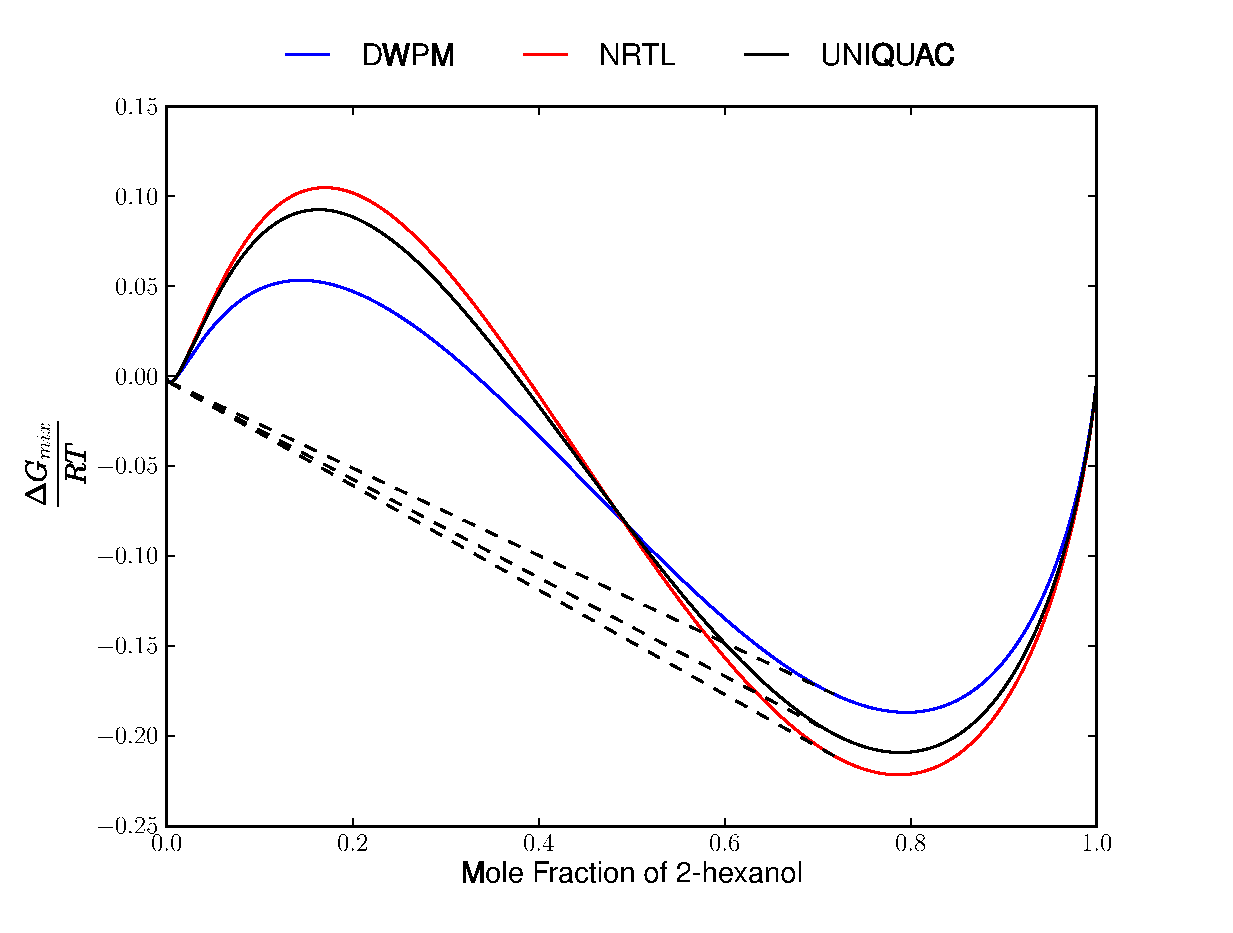
\includegraphics[width = \textwidth]{Results_Parts/BinaryParams/2-hexanol-water/AllModelsGibbsPlots/T_293.eps}
	\caption{293~$\mathrm{K}$} 
\end{subfigure}%
~%
\begin{subfigure}[h]{0.5\textwidth}
	\centering
	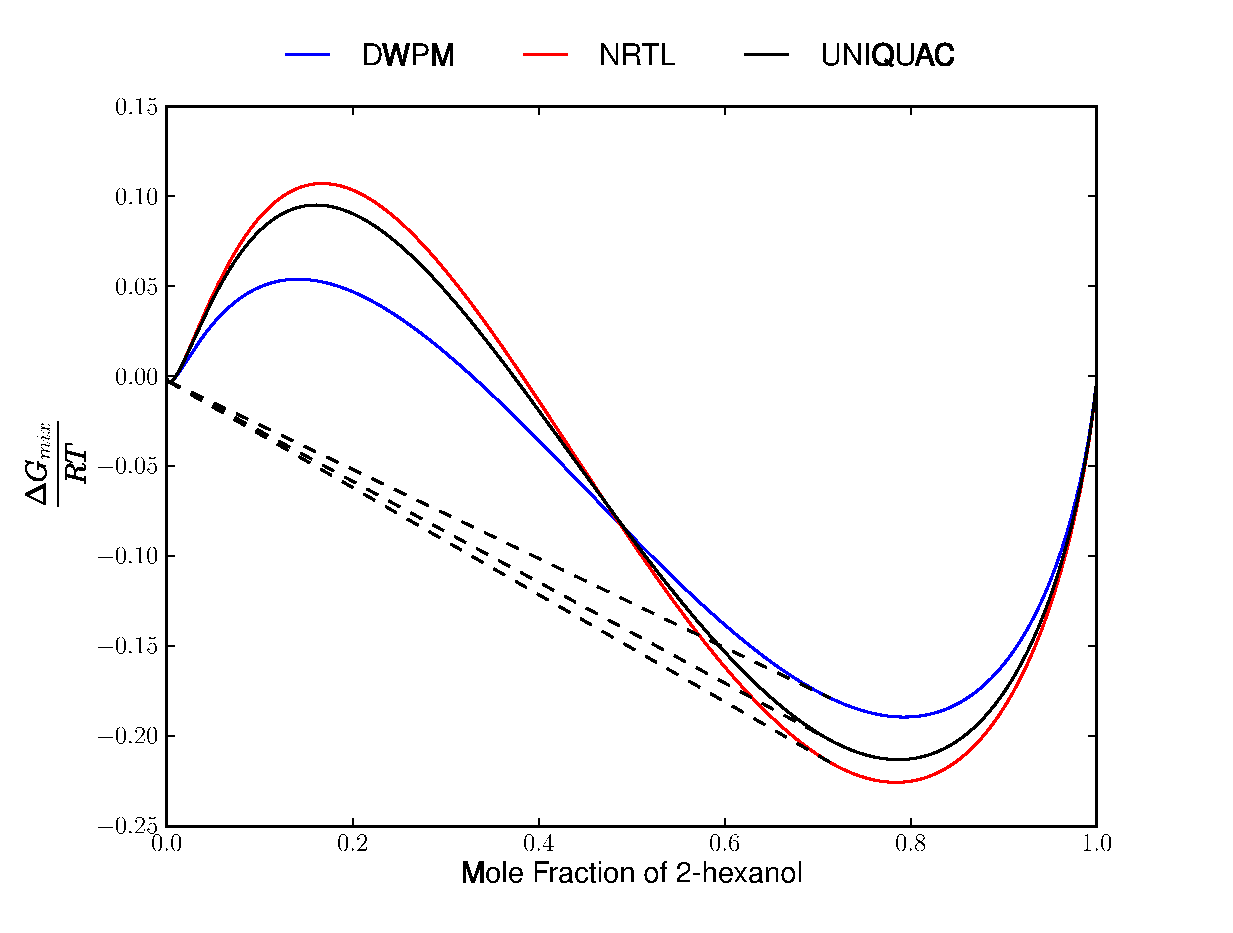
\includegraphics[width = \textwidth]{Results_Parts/BinaryParams/2-hexanol-water/AllModelsGibbsPlots/T_298.eps}
	\caption{298~$\mathrm{K}$}
\end{subfigure}%
\\%
\begin{subfigure}[h]{0.5\textwidth}
	\centering
	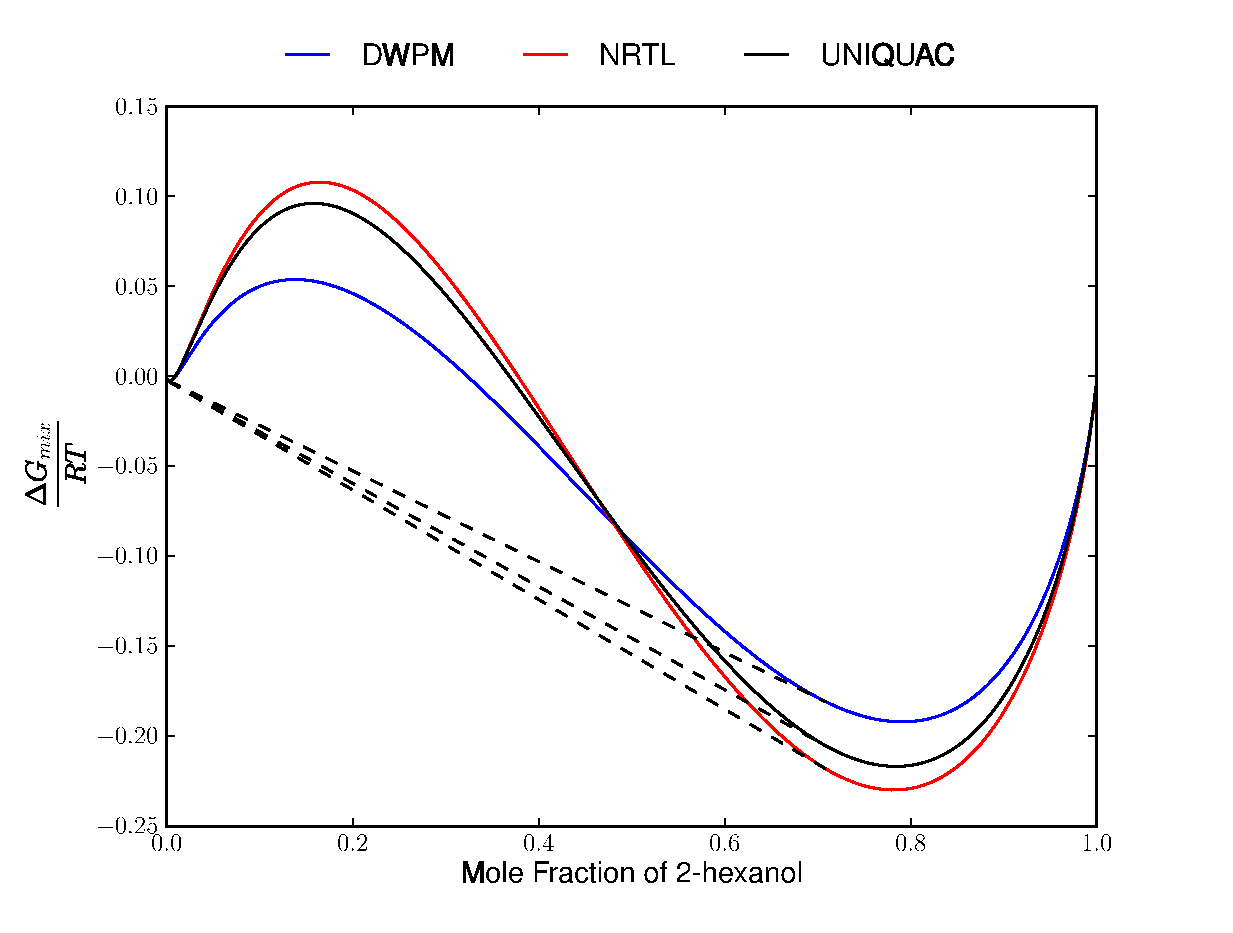
\includegraphics[width = \textwidth]{Results_Parts/BinaryParams/2-hexanol-water/AllModelsGibbsPlots/T_303.eps}
	\caption{303~$\mathrm{K}$} 
\end{subfigure}%
\caption{Calculated liquid-liquid equilibrium for 2-Hexanol and Water}
\end{figure}
\clearpage
%%------------------------------------------------------------------------------------------------------------------------------------------------%%
\subsection{13-Dimethyl Benzene and Water}
\vspace*{\fill}
\begin{figure}[hp]
\begin{subfigure}[h]{0.5\textwidth}
	\centering
	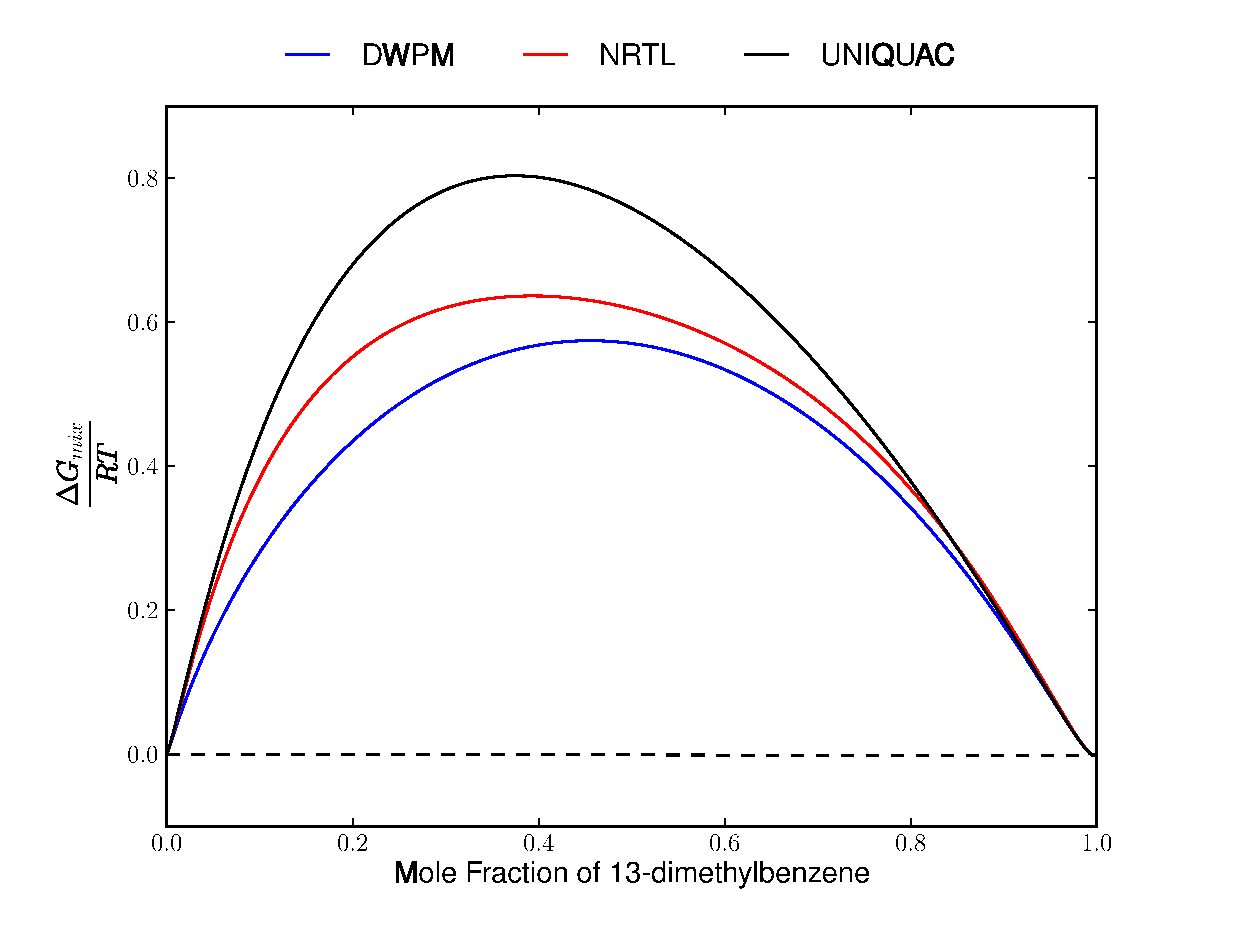
\includegraphics[width = \textwidth]{Results_Parts/BinaryParams/13-dimethylbenzene-water/AllModelsGibbsPlots/T_292.85.eps}
	\caption{292.85~$\mathrm{K}$} 
\end{subfigure}%
~%
\begin{subfigure}[h]{0.5\textwidth}
	\centering
	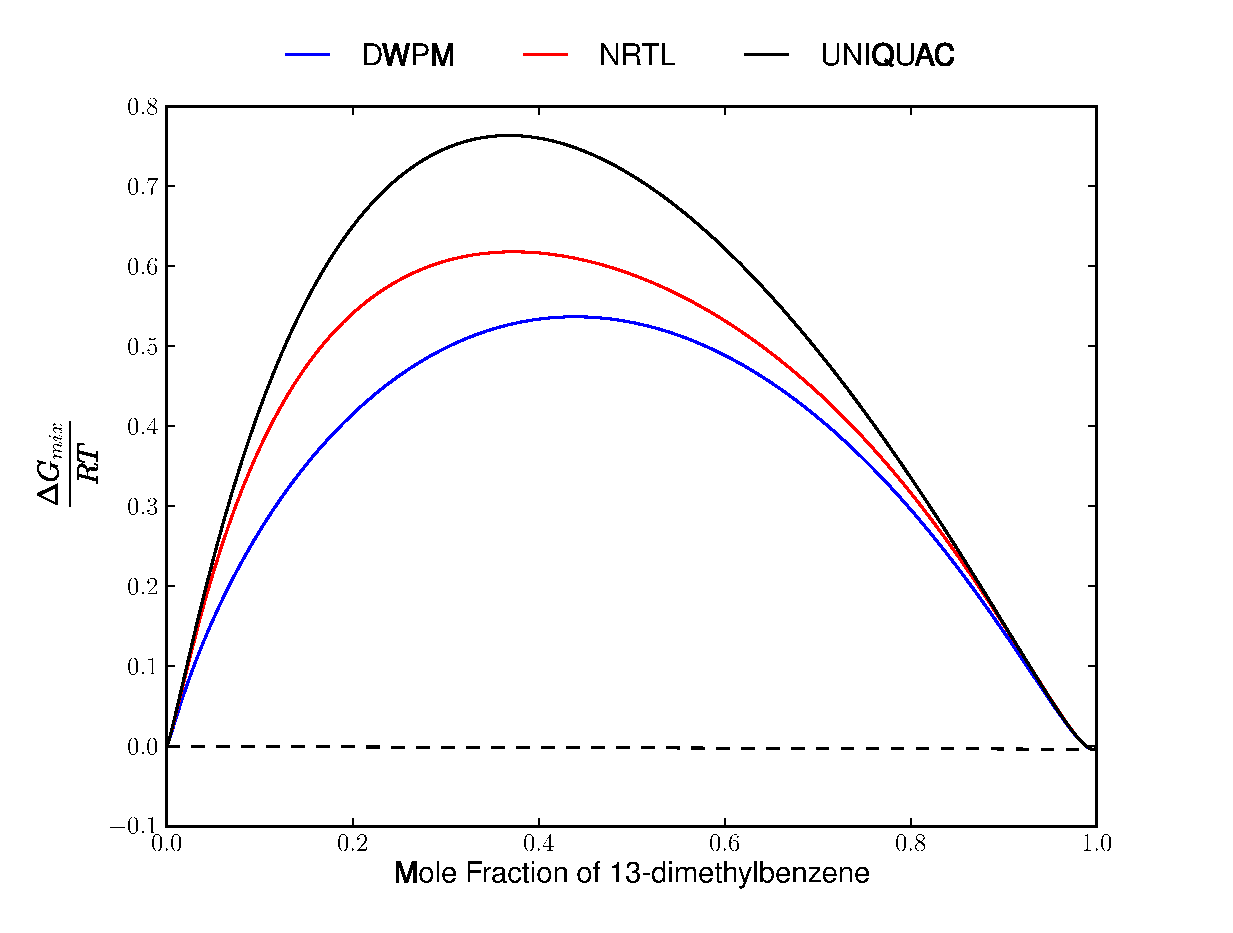
\includegraphics[width = \textwidth]{Results_Parts/BinaryParams/13-dimethylbenzene-water/AllModelsGibbsPlots/T_312.85.eps}
	\caption{312.85~$\mathrm{K}$} 
\end{subfigure}%
\\%
\begin{subfigure}[h]{0.5\textwidth}
\centering
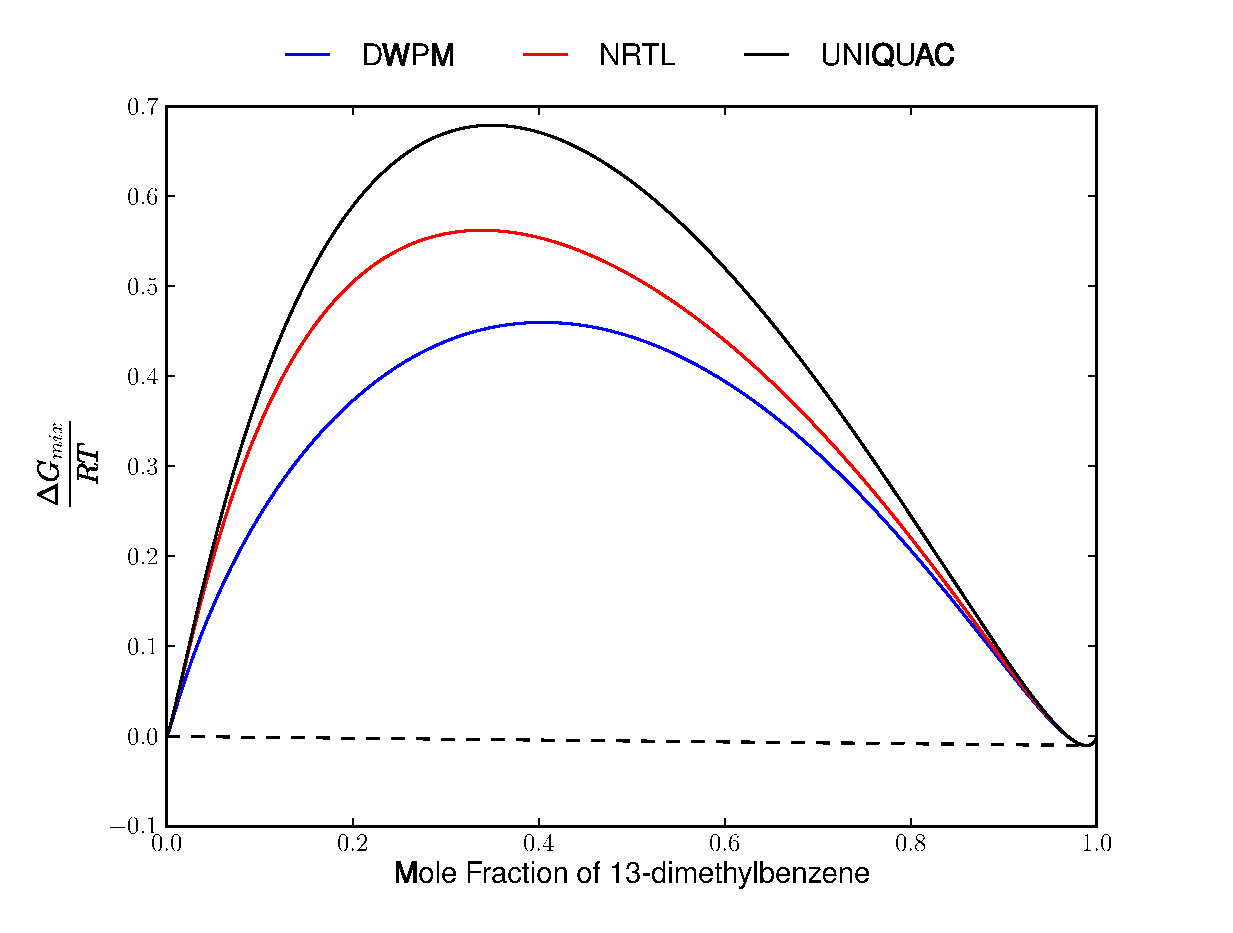
\includegraphics[width = \textwidth]{Results_Parts/BinaryParams/13-dimethylbenzene-water/AllModelsGibbsPlots/T_342.85.eps}
\caption{342.85~$\mathrm{K}$} 
\end{subfigure}%
\caption{Calculated liquid-liquid equilibrium for 13-Dimethyl Benzene and Water}
\end{figure}
\vspace*{\fill}
\clearpage
%%-------------------------------------------------------------------------------------------------------------------------------------------------%%
\subsection{Aniline and Water}
\vspace*{\fill}
\begin{figure}[hp]
\begin{subfigure}[h]{0.5\textwidth}
	\centering
	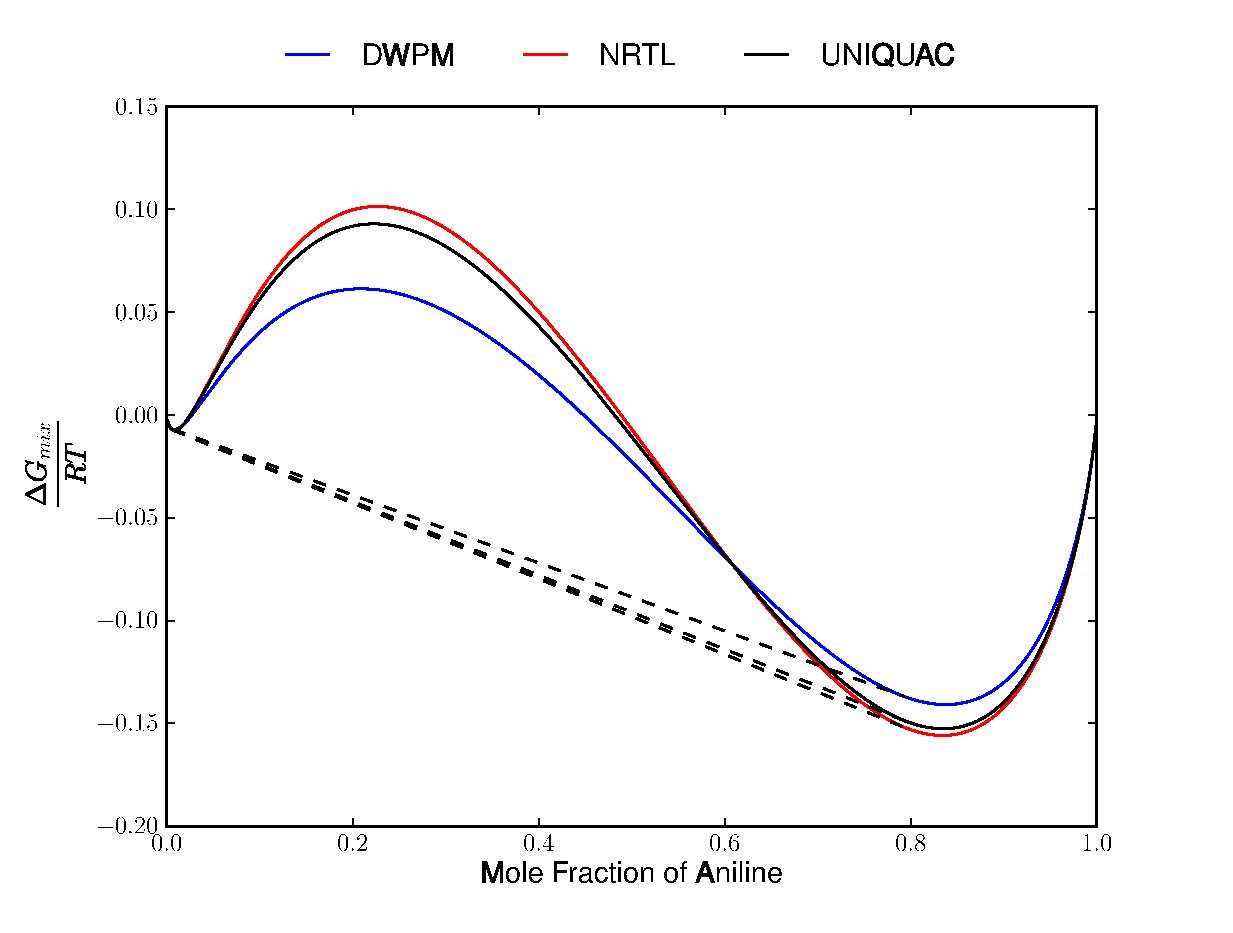
\includegraphics[width = \textwidth]{Results_Parts/BinaryParams/aniline-water/AllModelsGibbsPlots/T_281.6.eps}
	\caption{281.6~$\mathrm{K}$} 
\end{subfigure}%
~%
\begin{subfigure}[h]{0.5\textwidth}
	\centering
	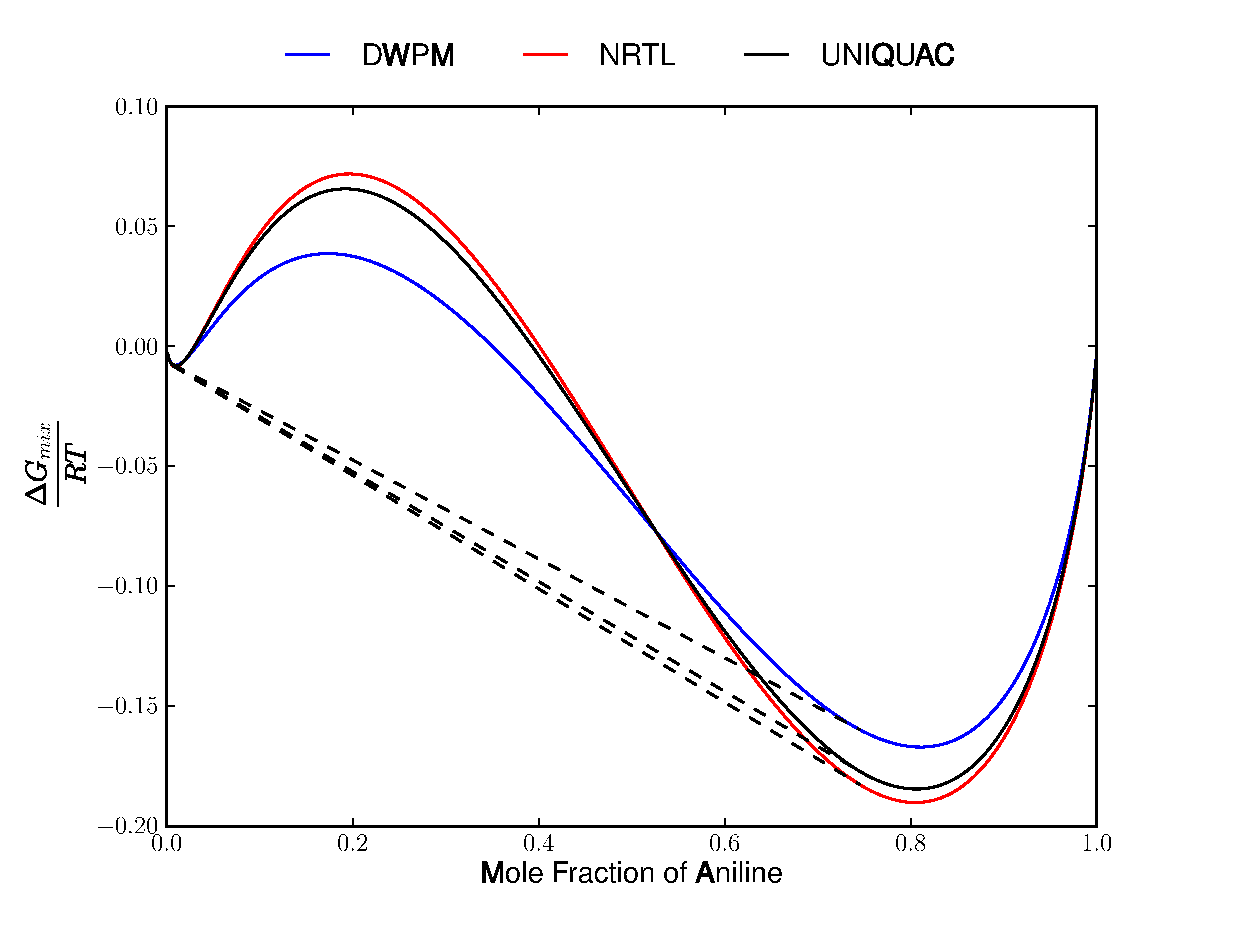
\includegraphics[width = \textwidth]{Results_Parts/BinaryParams/aniline-water/AllModelsGibbsPlots/T_298.4.eps}
	\caption{298.4~$\mathrm{K}$} 
\end{subfigure}%
\\%
\begin{subfigure}[h]{0.5\textwidth}
	\centering
	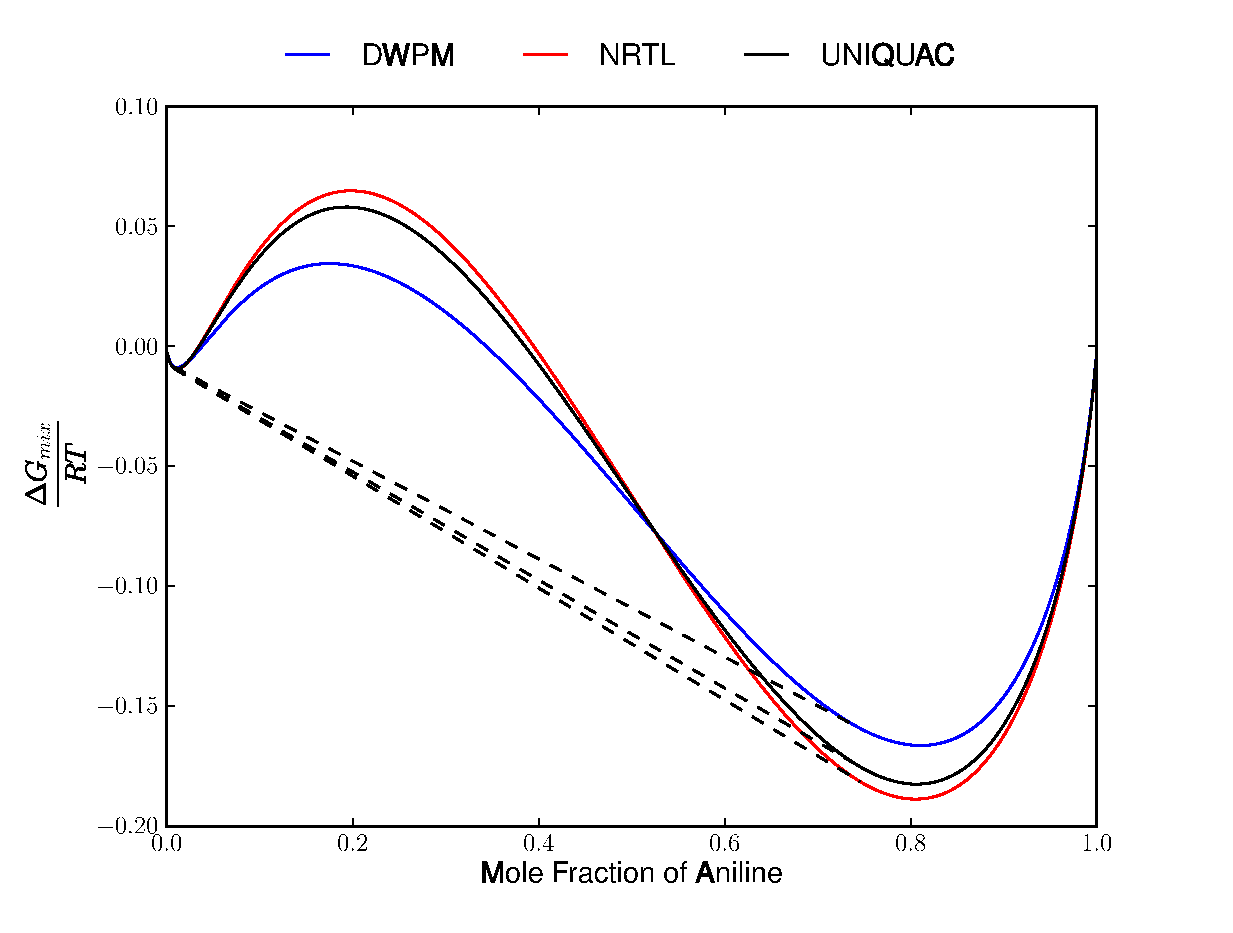
\includegraphics[width = \textwidth]{Results_Parts/BinaryParams/aniline-water/AllModelsGibbsPlots/T_321.0.eps}
	\caption{321.0~$\mathrm{K}$} 
\end{subfigure}%
~%
\begin{subfigure}[h]{0.5\textwidth}
	\centering
	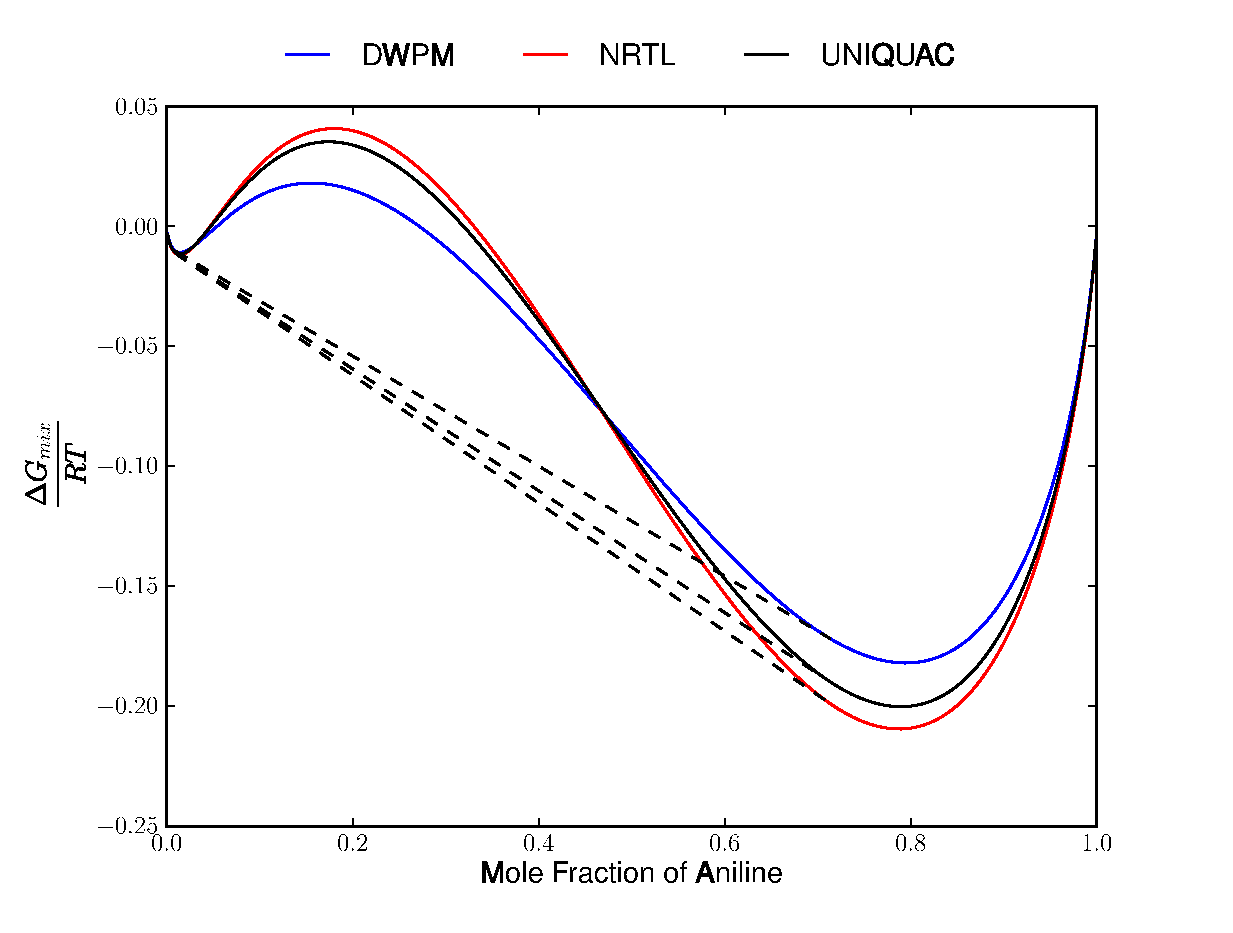
\includegraphics[width = \textwidth]{Results_Parts/BinaryParams/aniline-water/AllModelsGibbsPlots/T_339.3.eps}
	\caption{339.3~$\mathrm{K}$} 
\end{subfigure}%
\caption{Calculated liquid-liquid equilibrium for Aniline and Water}
\end{figure}
\vspace*{\fill}
\clearpage
\begin{figure}[hpt]
\ContinuedFloat 
\begin{subfigure}[h]{0.5\textwidth}
\centering
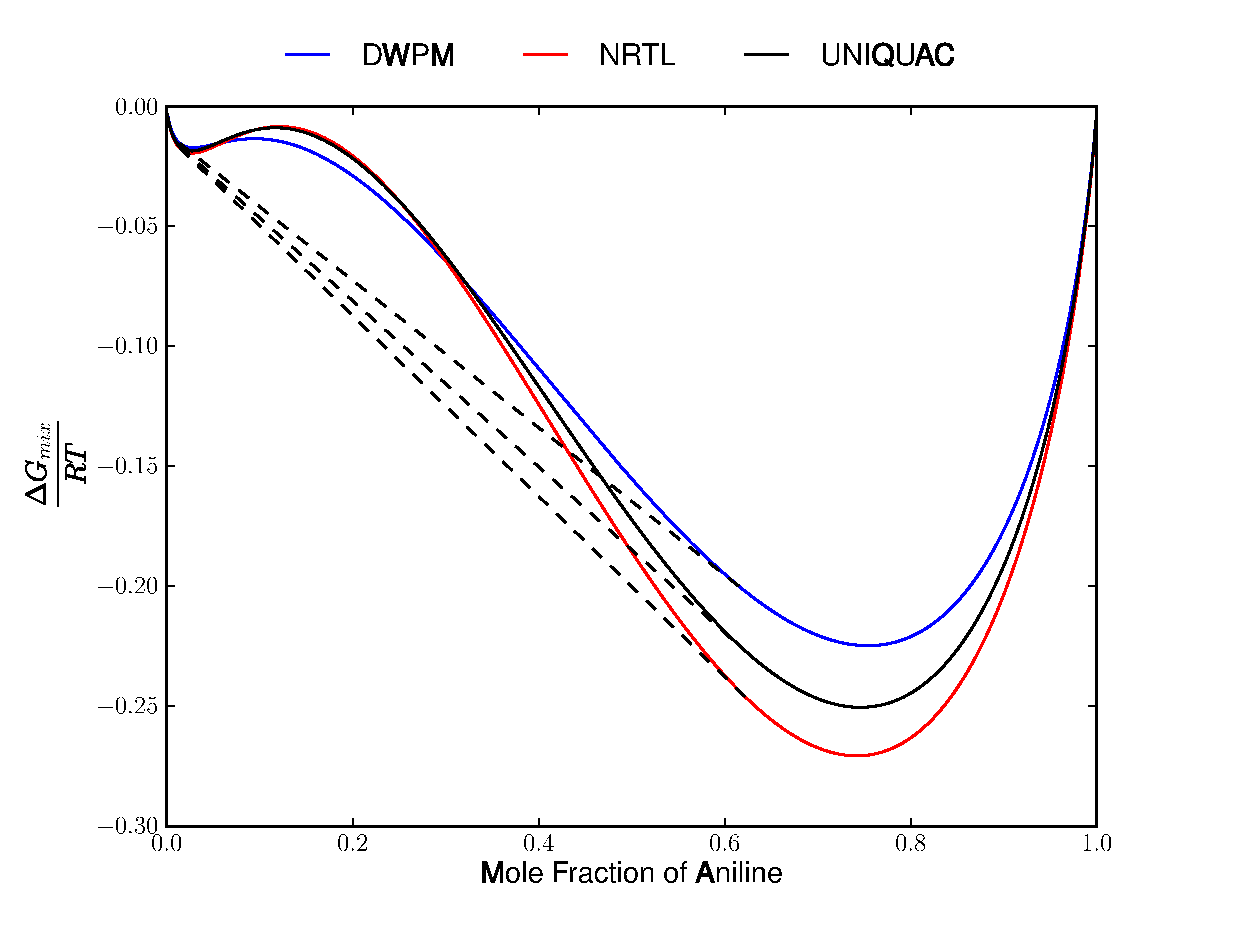
\includegraphics[width = \textwidth]{Results_Parts/BinaryParams/aniline-water/AllModelsGibbsPlots/T_369.7.eps}
\caption{369.7~$\mathrm{K}$}
\end{subfigure}%
\caption[]{Calculated liquid-liquid equilibrium for Aniline and Water}
\end{figure}
\clearpage

%%-------------------------------------------------------------------------------------------------------------------------------------------------%%

\subsection{Diethylene Glycol and 12-Dimethyl Benzene}
\vspace*{\fill}
\begin{figure}[hp]
\begin{subfigure}[h]{0.5\textwidth}
	\centering
	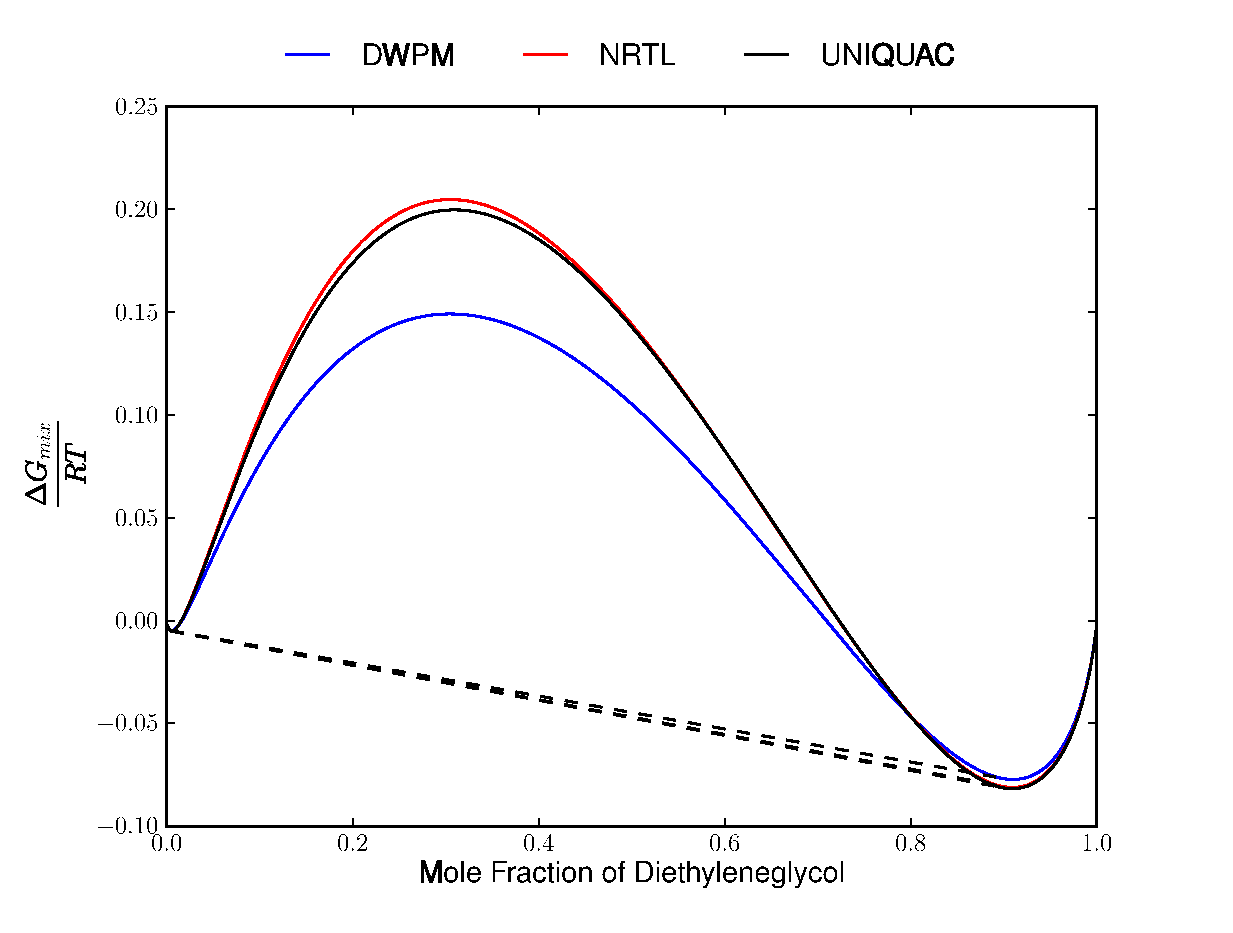
\includegraphics[width = \textwidth]{Results_Parts/BinaryParams/diethyleneglycol-12-dimethylbenzene/AllModelsGibbsPlots/T_313.3.eps}
	\caption{313.3~$\mathrm{K}$} 
\end{subfigure}%
~%
\begin{subfigure}[h]{0.5\textwidth}
	\centering
	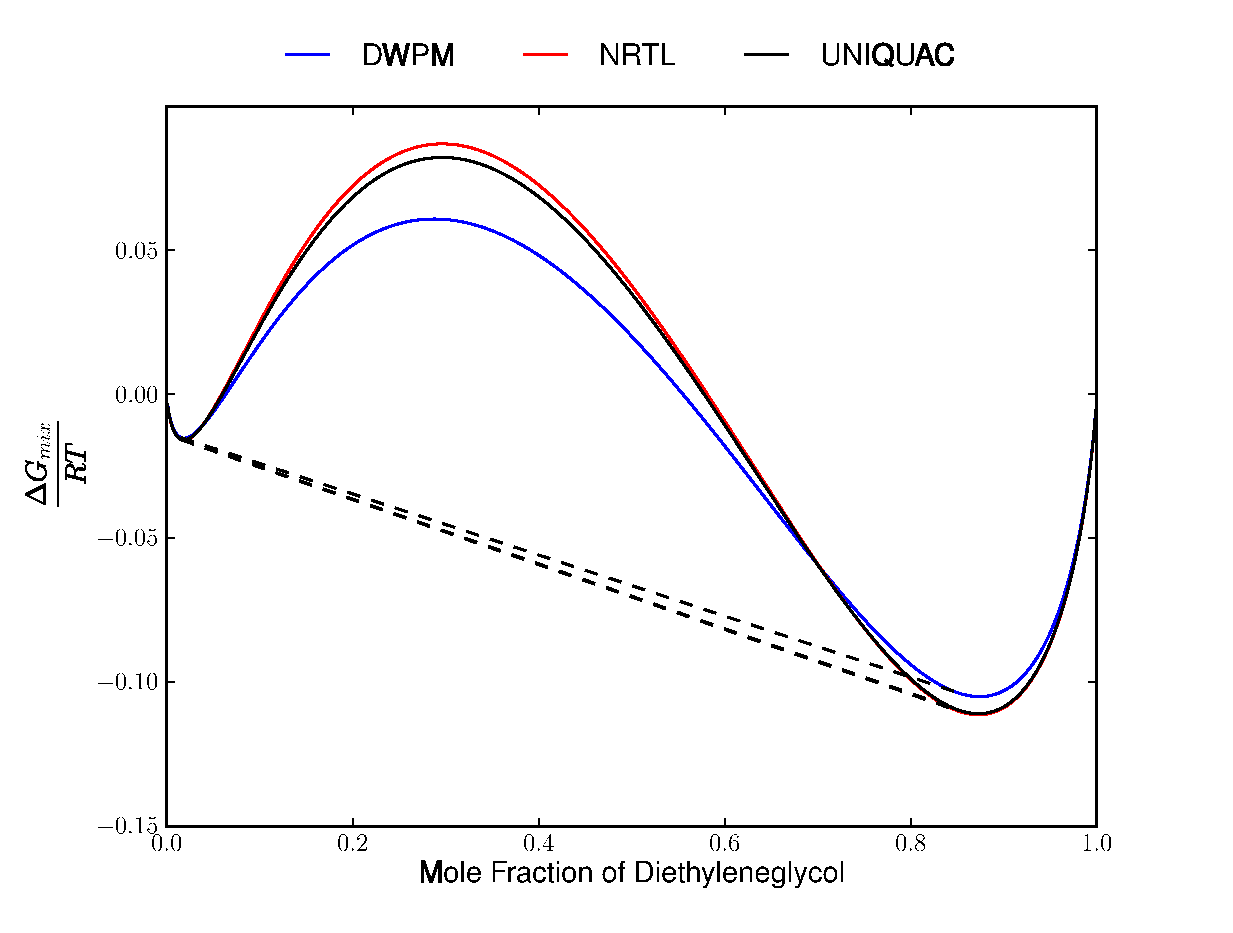
\includegraphics[width = \textwidth]{Results_Parts/BinaryParams/diethyleneglycol-12-dimethylbenzene/AllModelsGibbsPlots/T_332.8.eps}
	\caption{332.8~$\mathrm{K}$} 
\end{subfigure}%
\\%
\begin{subfigure}[h]{0.5\textwidth}
	\centering
	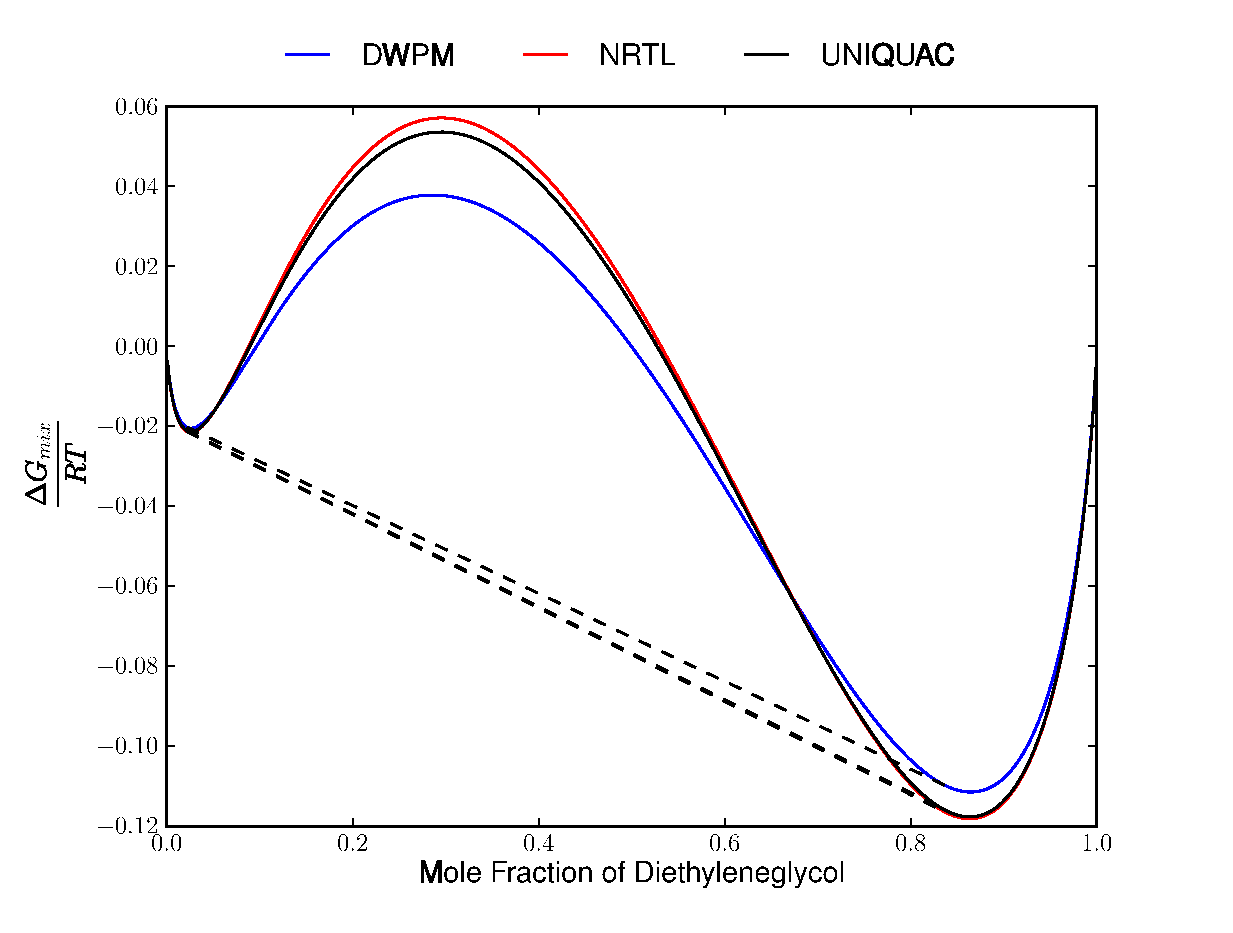
\includegraphics[width = \textwidth]{Results_Parts/BinaryParams/diethyleneglycol-12-dimethylbenzene/AllModelsGibbsPlots/T_353.8.eps}
	\caption{383.8~$\mathrm{K}$} 
\end{subfigure}%
~%
\begin{subfigure}[h]{0.5\textwidth}
	\centering
	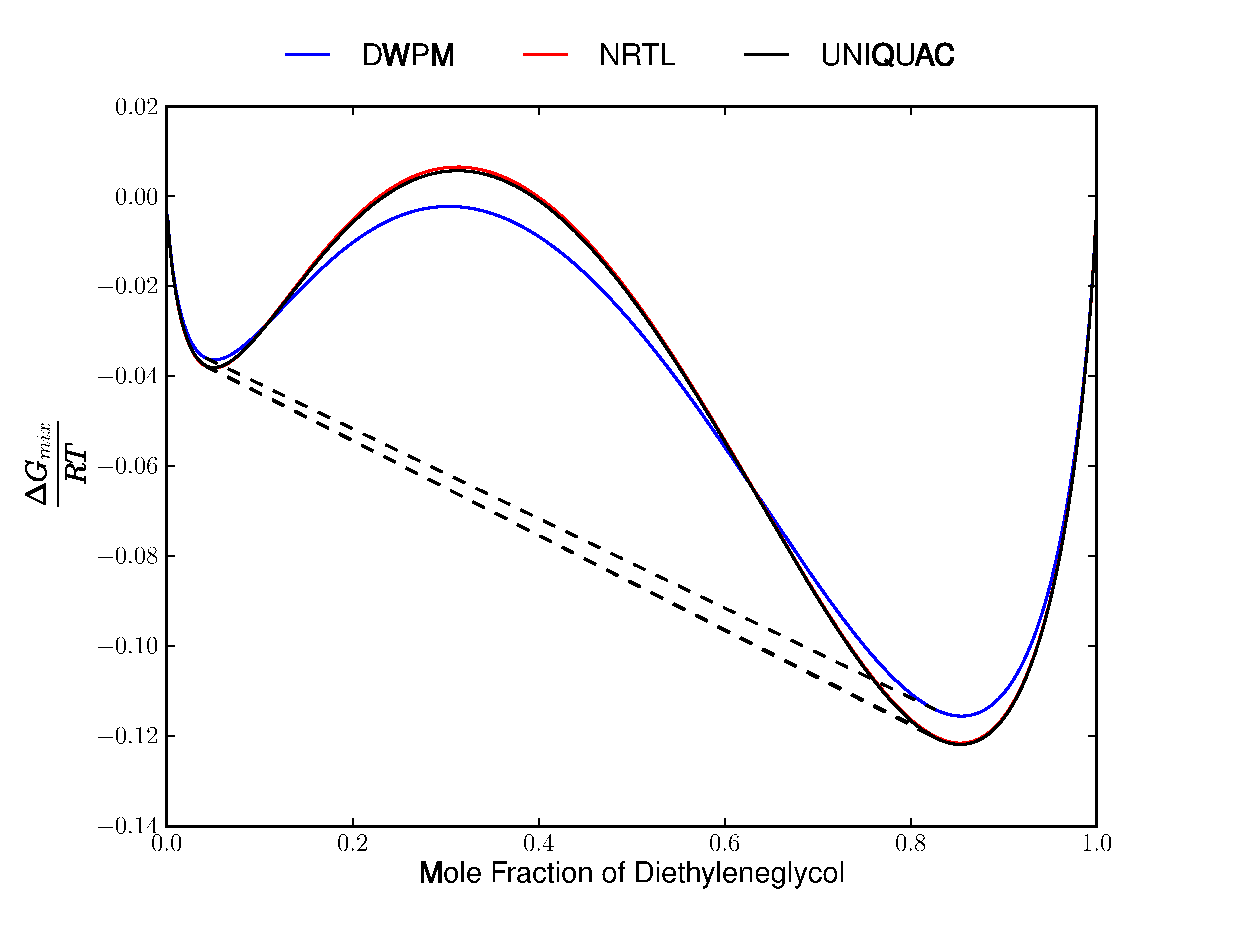
\includegraphics[width = \textwidth]{Results_Parts/BinaryParams/diethyleneglycol-12-dimethylbenzene/AllModelsGibbsPlots/T_363.0.eps}
	\caption{363.0~$\mathrm{K}$} 
\end{subfigure}%
\caption{Calculated liquid-liquid equilibrium for Diethylene Glycol and 12-Dimethyl Benzene}
\end{figure}
\vspace*{\fill}
\clearpage
\begin{figure}[hpt]
\ContinuedFloat 
\begin{subfigure}[h]{0.5\textwidth}
	\centering
	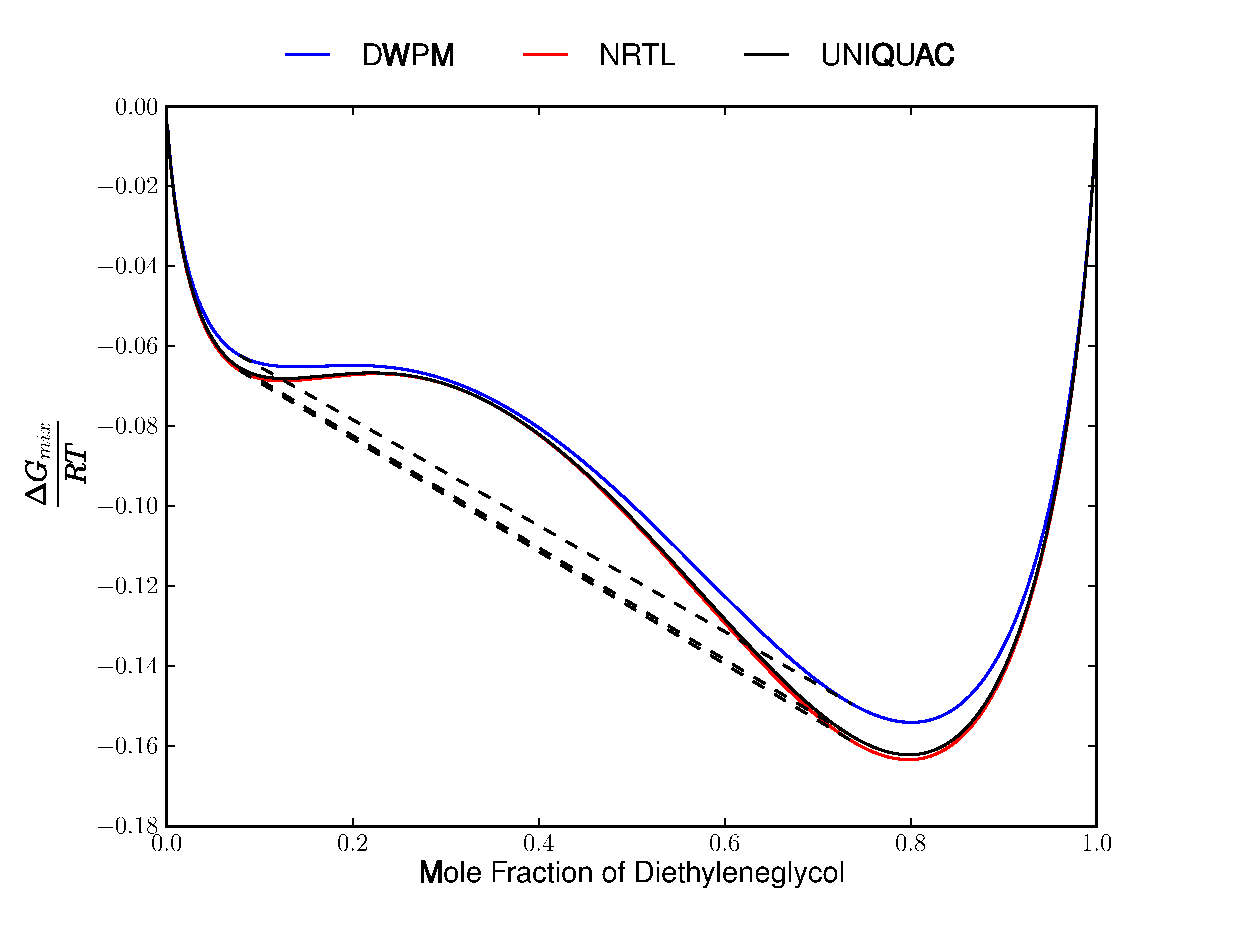
\includegraphics[width = \textwidth]{Results_Parts/BinaryParams/diethyleneglycol-12-dimethylbenzene/AllModelsGibbsPlots/T_393.0.eps}
	\caption{393.0~$\mathrm{K}$} 
\end{subfigure}
\caption[]{Calculated liquid-liquid equilibrium for Diethylene Glycol and 12-Dimethyl Benzene}
\end{figure}
\clearpage

%%------------------------------------------------------------------------------------------------------------------------------------------------%%

\subsection{Dipropyl Ether and Water}
\vspace*{\fill}
\begin{figure}[hp]
\begin{subfigure}[h]{0.5\textwidth}
	\centering
	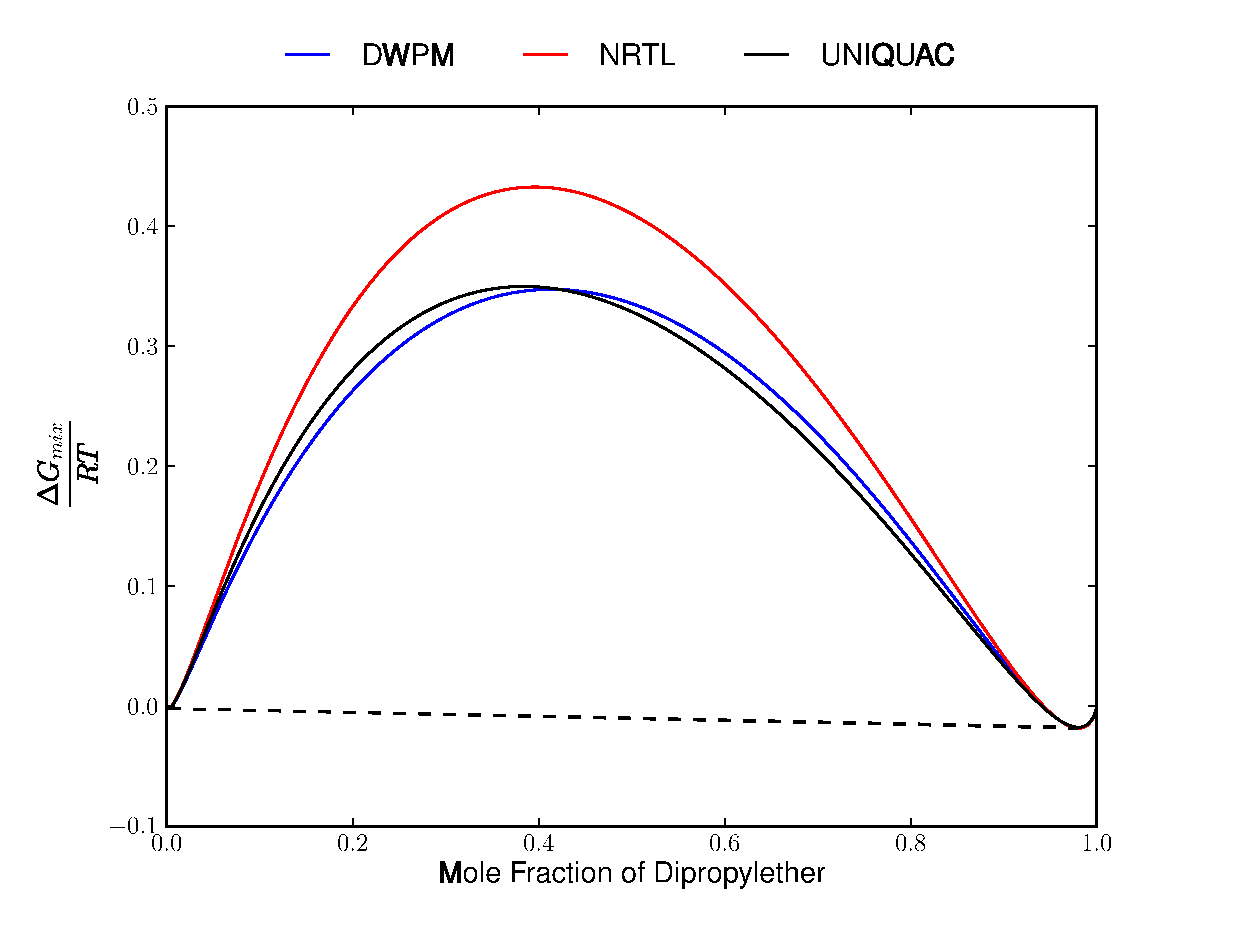
\includegraphics[width = \textwidth]{Results_Parts/BinaryParams/dipropylether-water/AllModelsGibbsPlots/T_273.eps}
	\caption{273.0~$\mathrm{K}$} 
\end{subfigure}%
~%
\begin{subfigure}[h]{0.5\textwidth}
	\centering
	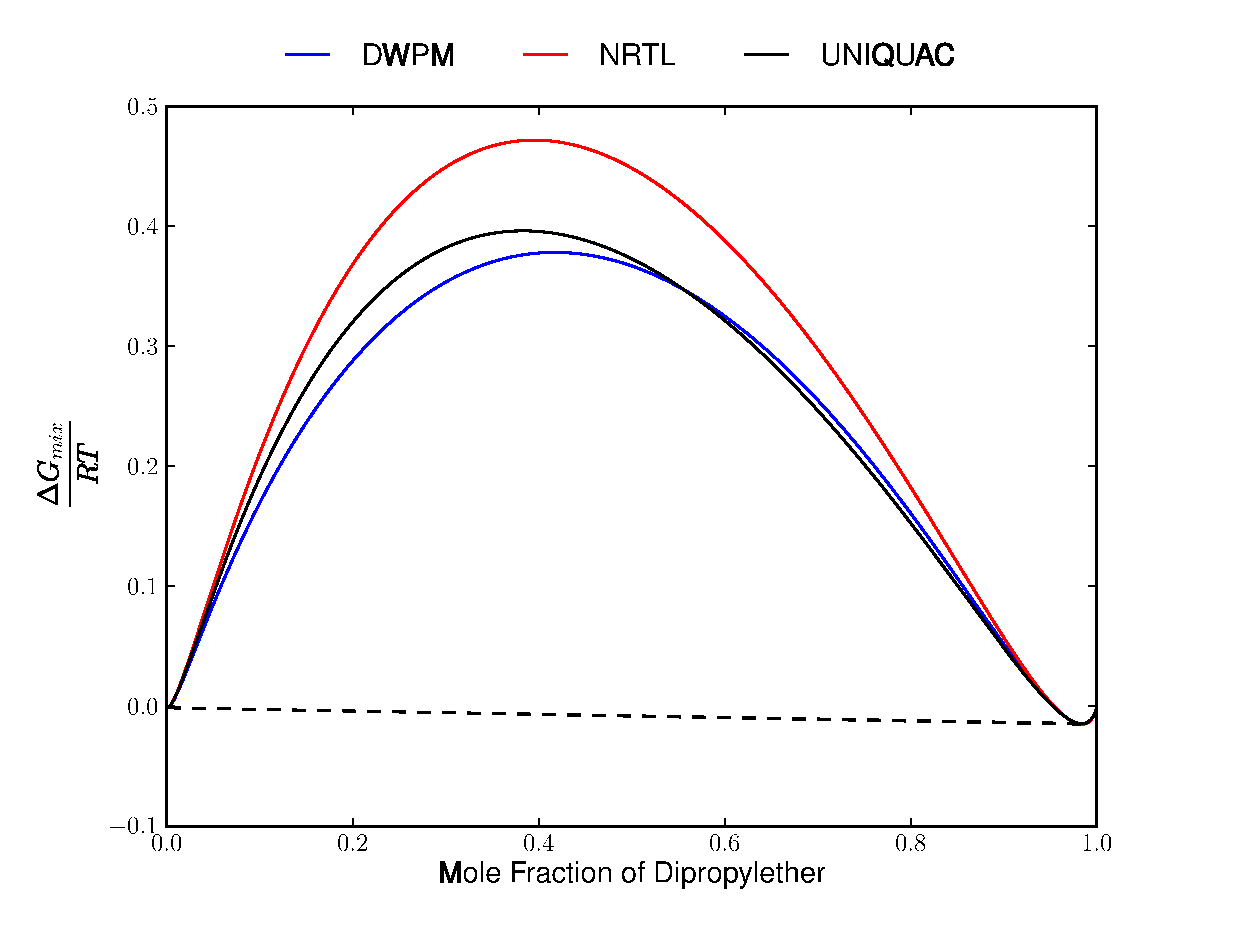
\includegraphics[width = \textwidth]{Results_Parts/BinaryParams/dipropylether-water/AllModelsGibbsPlots/T_283.eps}
	\caption{283.0~$\mathrm{K}$} 
\end{subfigure}%
\\%
\begin{subfigure}[h]{0.5\textwidth}
	\centering
	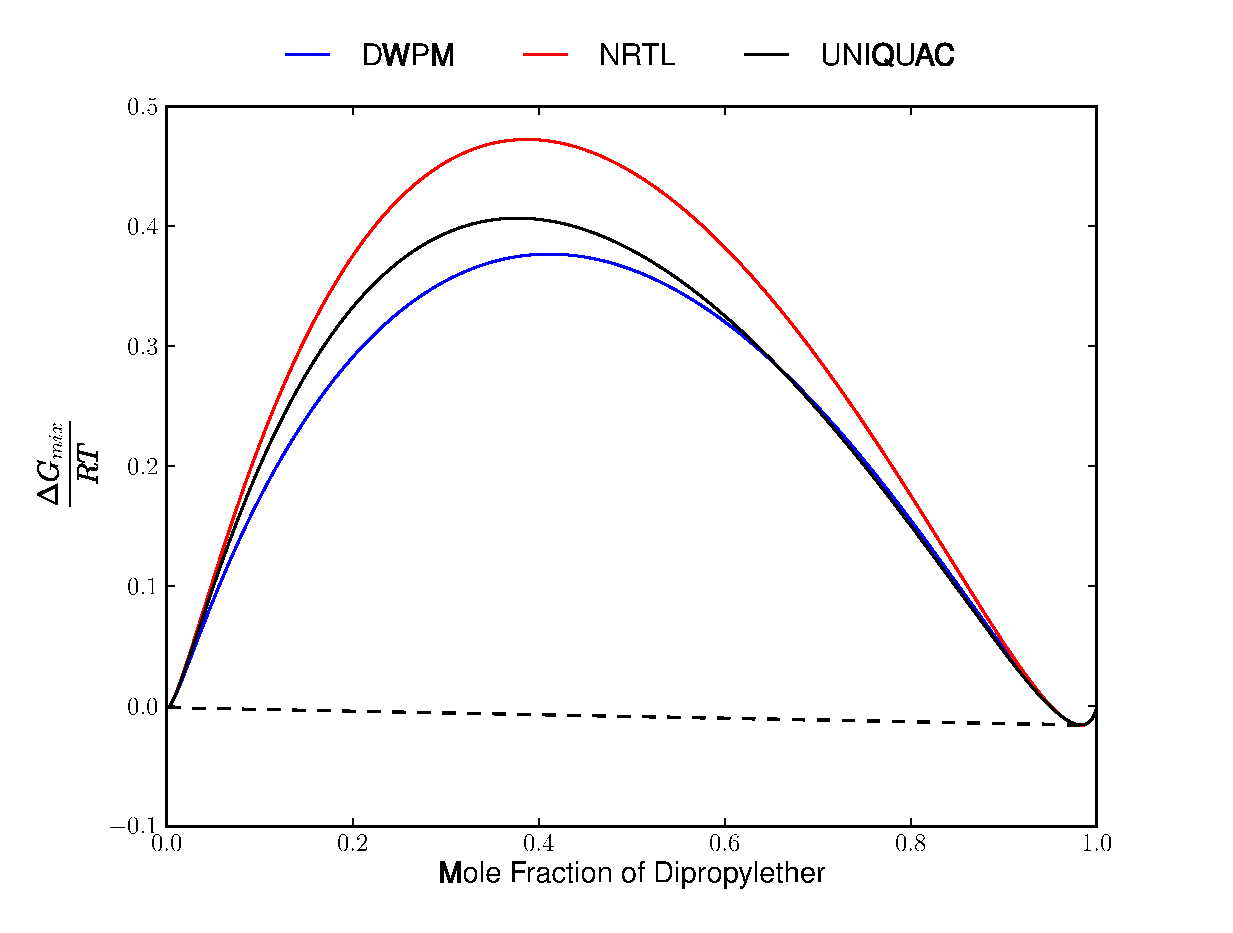
\includegraphics[width = \textwidth]{Results_Parts/BinaryParams/dipropylether-water/AllModelsGibbsPlots/T_288.eps}
	\caption{288.0~$\mathrm{K}$} 
\end{subfigure}%
~%
\begin{subfigure}[h]{0.5\textwidth}
	\centering
	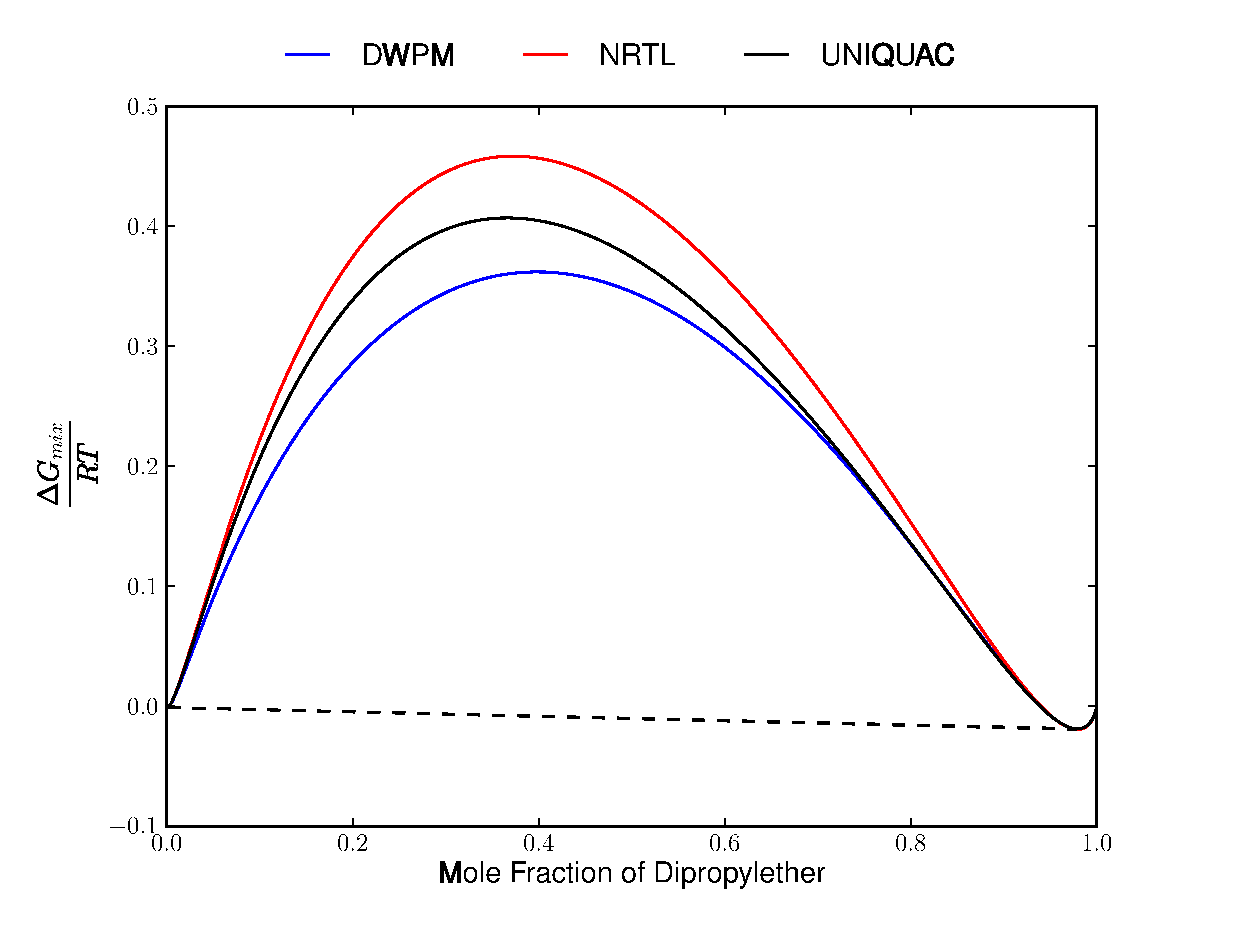
\includegraphics[width = \textwidth]{Results_Parts/BinaryParams/dipropylether-water/AllModelsGibbsPlots/T_293.eps}
	\caption{293.0~$\mathrm{K}$} 
\end{subfigure}%
\caption{Calculated liquid-liquid equilibrium for Dipropyl Ether and Water}
\end{figure}
\vspace*{\fill}
\clearpage
\begin{figure}[hpt]
\ContinuedFloat 
\begin{subfigure}[h]{0.5\textwidth}
	\centering
	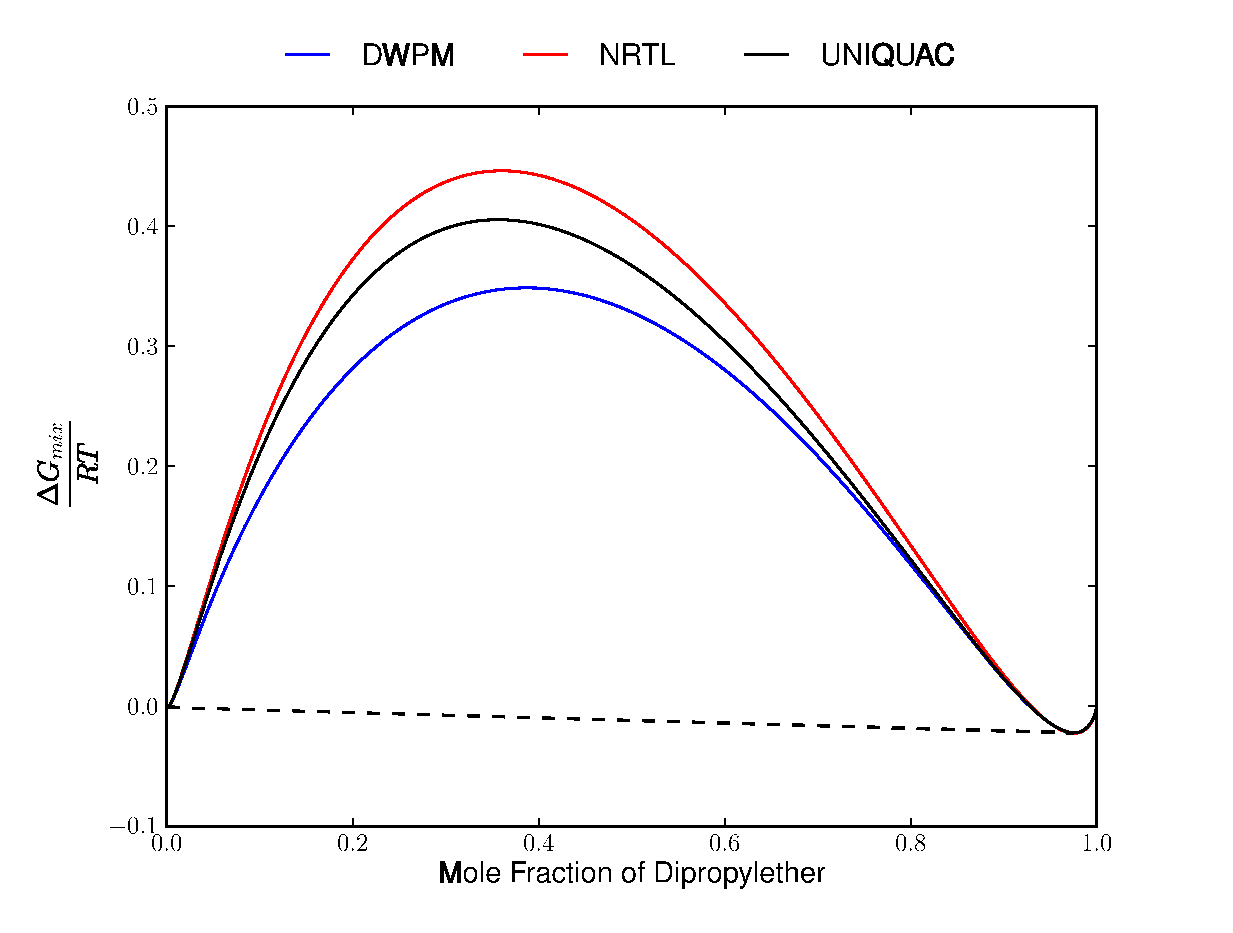
\includegraphics[width = \textwidth]{Results_Parts/BinaryParams/dipropylether-water/AllModelsGibbsPlots/T_298.eps}
	\caption{298.0~$\mathrm{K}$}
\end{subfigure}%
\caption[]{Calculated liquid-liquid equilibrium for Dipropyl Ether and Water}
\end{figure}
\clearpage

%%------------------------------------------------------------------------------------------------------------------------------------------------%%

\subsection{Ethyl Ester Acetic Acid and Water}
\vspace*{\fill}
\begin{figure}[hp]
\begin{subfigure}[h]{0.5\textwidth}
	\centering
	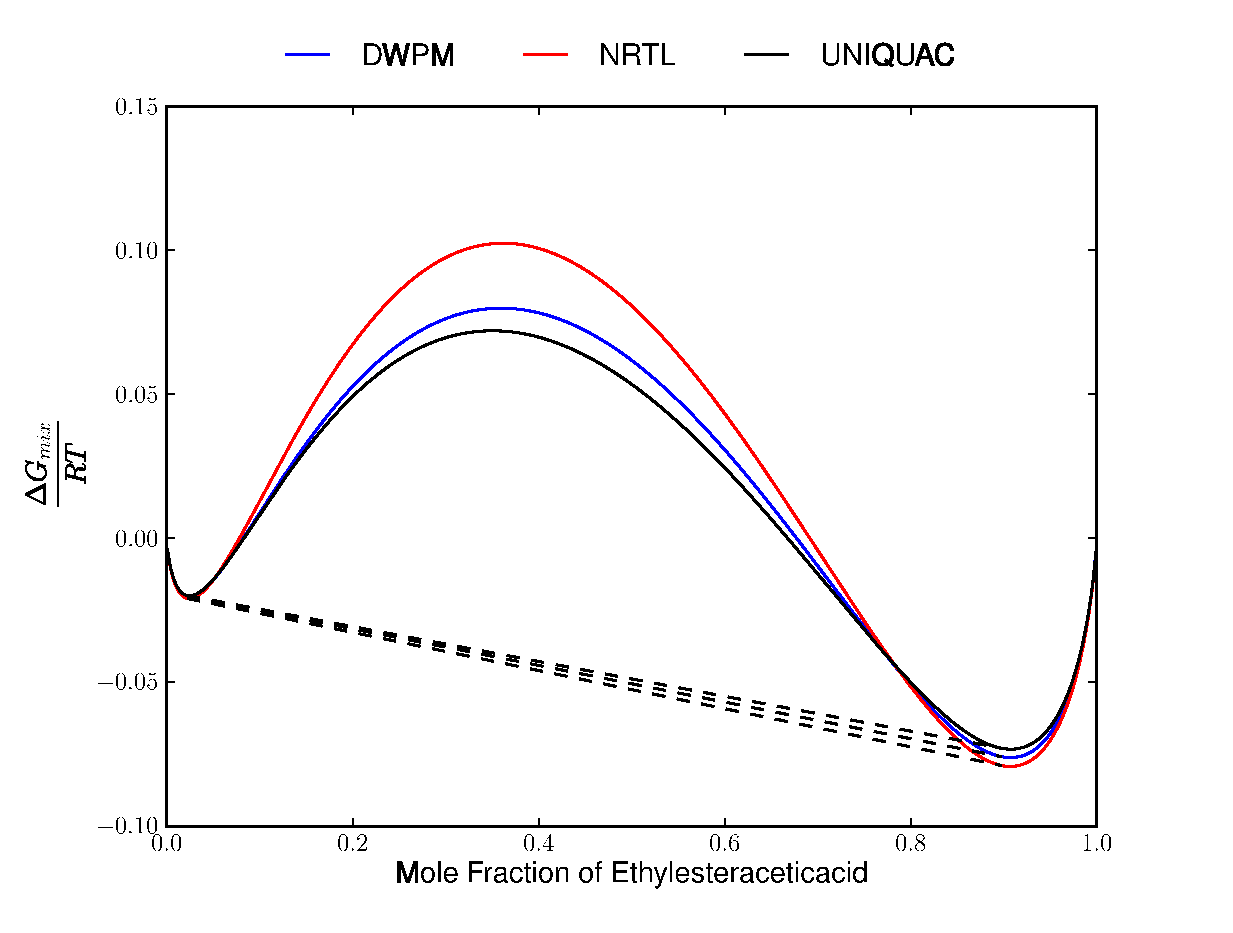
\includegraphics[width = \textwidth]{Results_Parts/BinaryParams/ethylesteraceticacid-water/AllModelsGibbsPlots/T_273.0.eps}
	\caption{273.0~$\mathrm{K}$} 
\end{subfigure}%
~%
\begin{subfigure}[h]{0.5\textwidth}
	\centering
	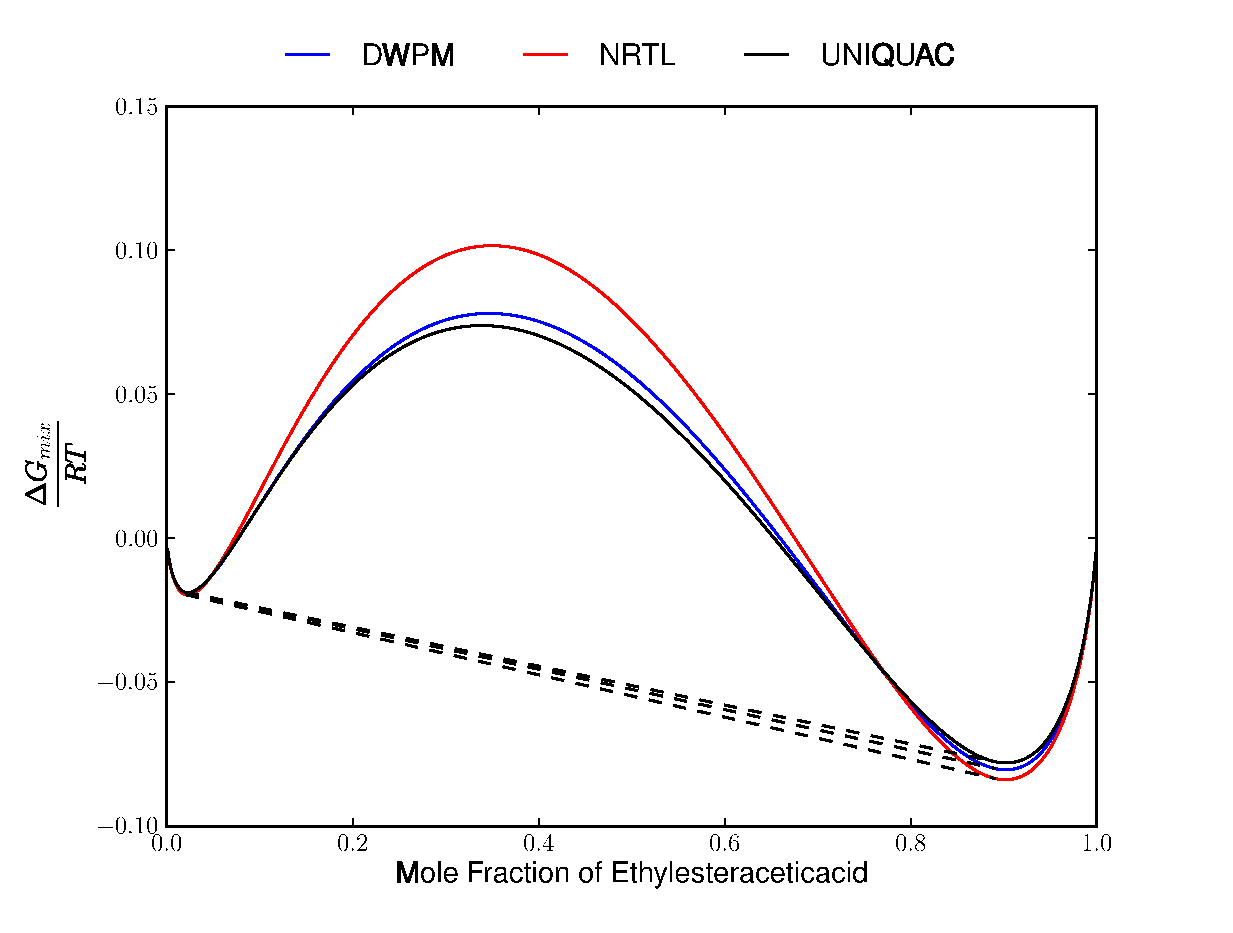
\includegraphics[width = \textwidth]{Results_Parts/BinaryParams/ethylesteraceticacid-water/AllModelsGibbsPlots/T_278.0.eps}
	\caption{278.0~$\mathrm{K}$} 
\end{subfigure}%
\\%
\begin{subfigure}[h]{0.5\textwidth}
	\centering
	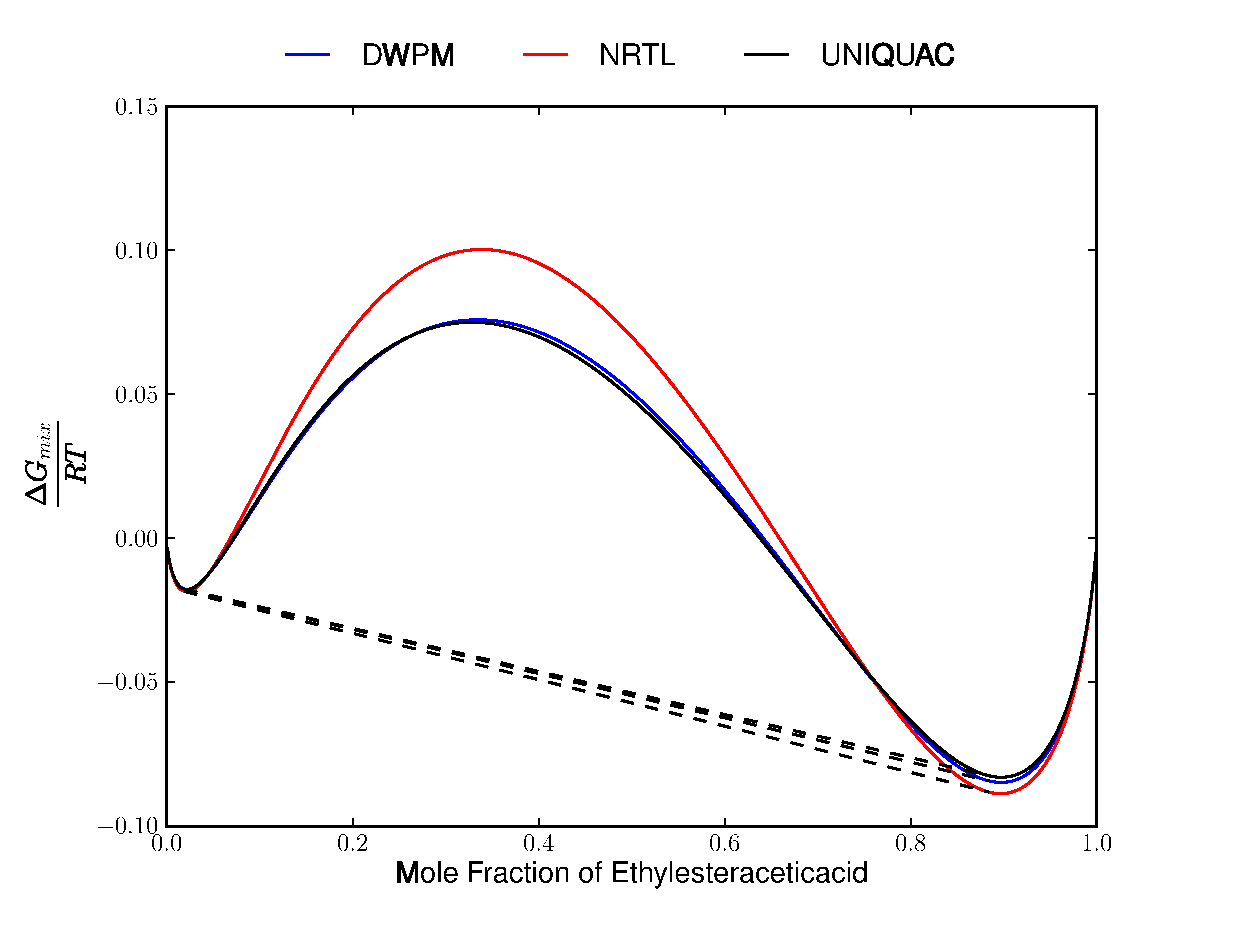
\includegraphics[width = \textwidth]{Results_Parts/BinaryParams/ethylesteraceticacid-water/AllModelsGibbsPlots/T_283.0.eps}
	\caption{283.0~$\mathrm{K}$}
\end{subfigure}%
~%
\begin{subfigure}[h]{0.5\textwidth}
	\centering
	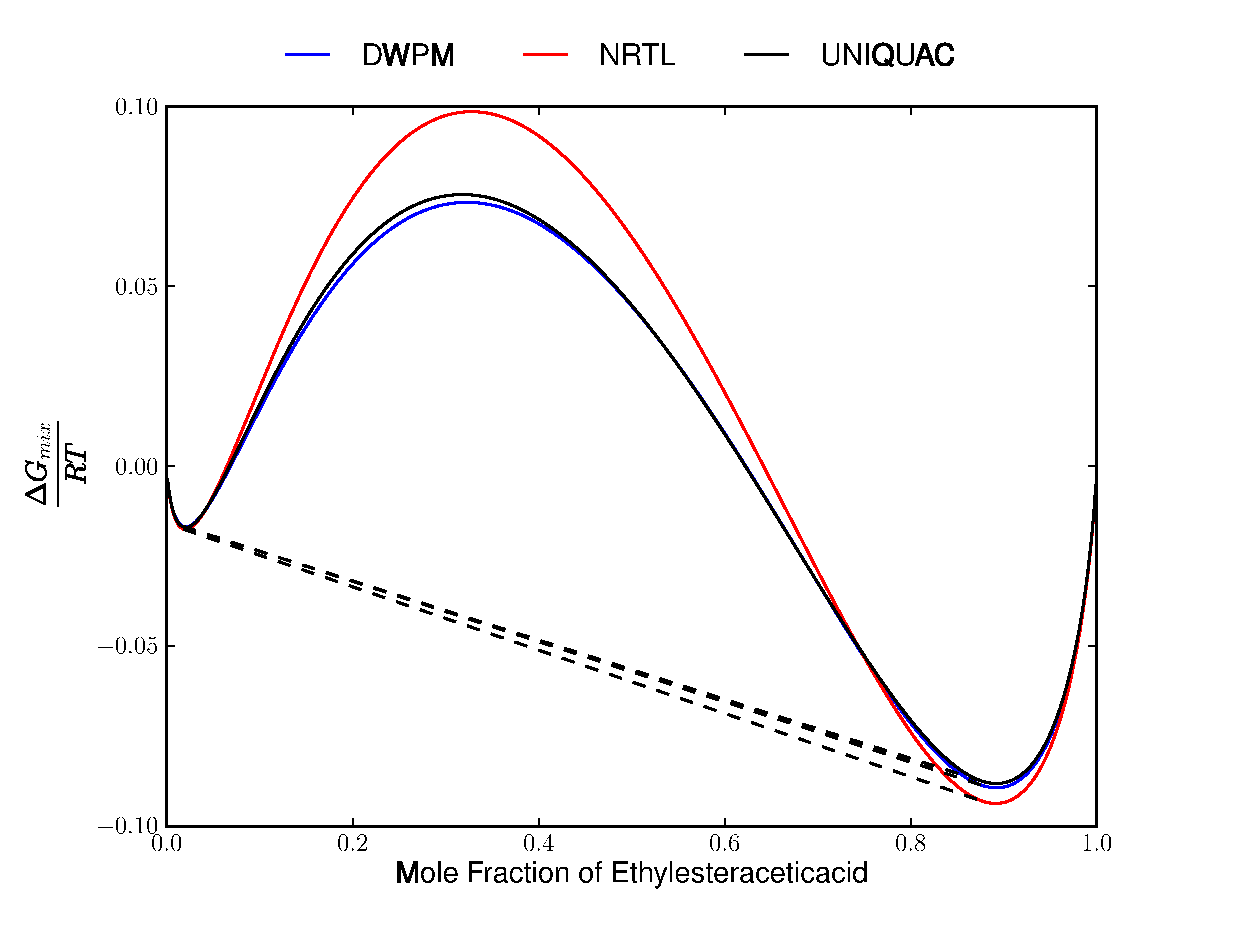
\includegraphics[width = \textwidth]{Results_Parts/BinaryParams/ethylesteraceticacid-water/AllModelsGibbsPlots/T_288.0.eps}
	\caption{288.0~$\mathrm{K}$}
\end{subfigure}%
\caption{Calculated liquid-liquid equilibrium for Ethyl Ester Acetic Acid and Water}
\end{figure}
\vspace*{\fill}
\clearpage
\vspace*{\fill}
\begin{figure}[hp]
\ContinuedFloat 
\begin{subfigure}[h]{0.5\textwidth}
	\centering
	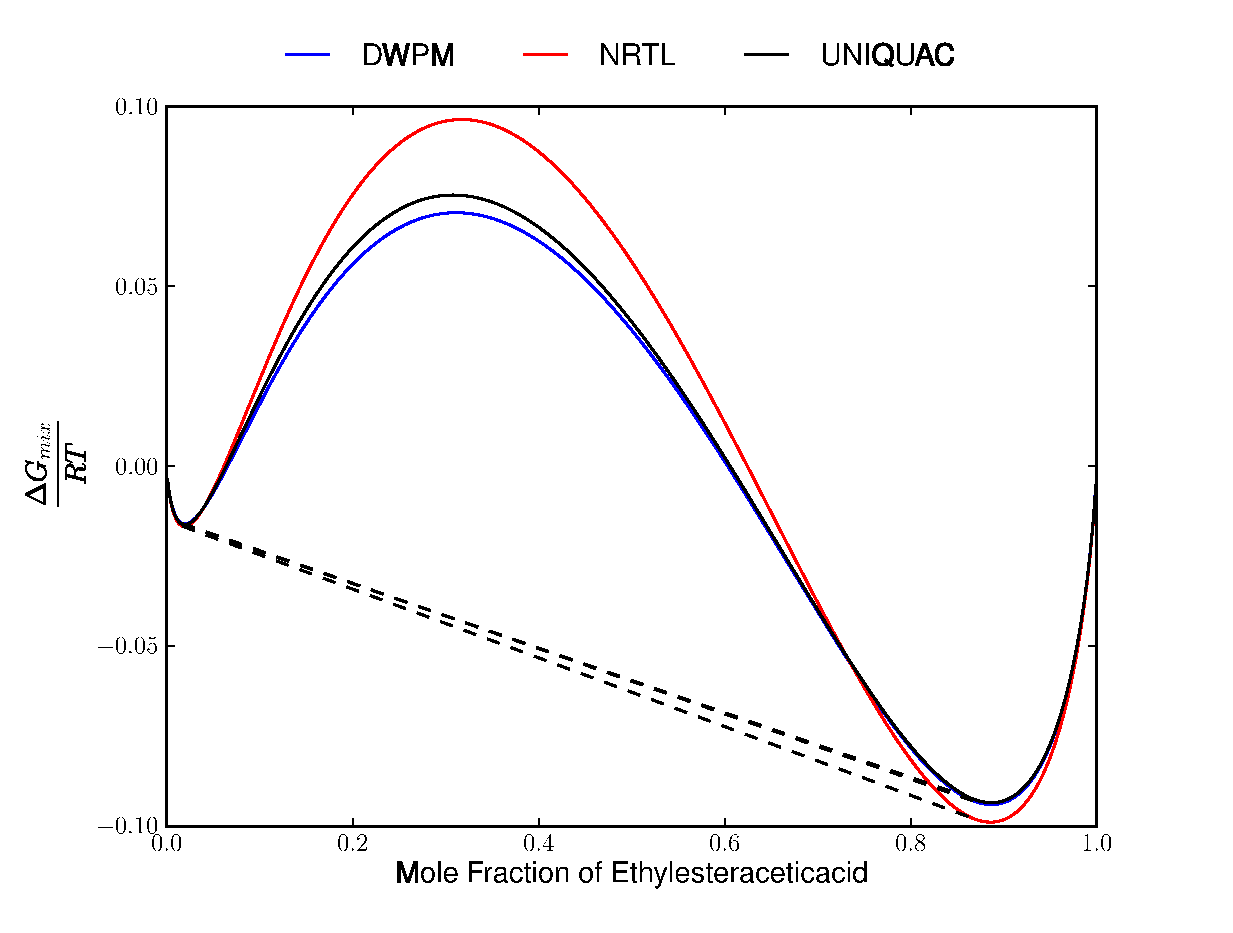
\includegraphics[width = \textwidth]{Results_Parts/BinaryParams/ethylesteraceticacid-water/AllModelsGibbsPlots/T_293.0.eps}
	\caption{293.0~$\mathrm{K}$}
\end{subfigure}%
~%
\begin{subfigure}[h]{0.5\textwidth}
	\centering
	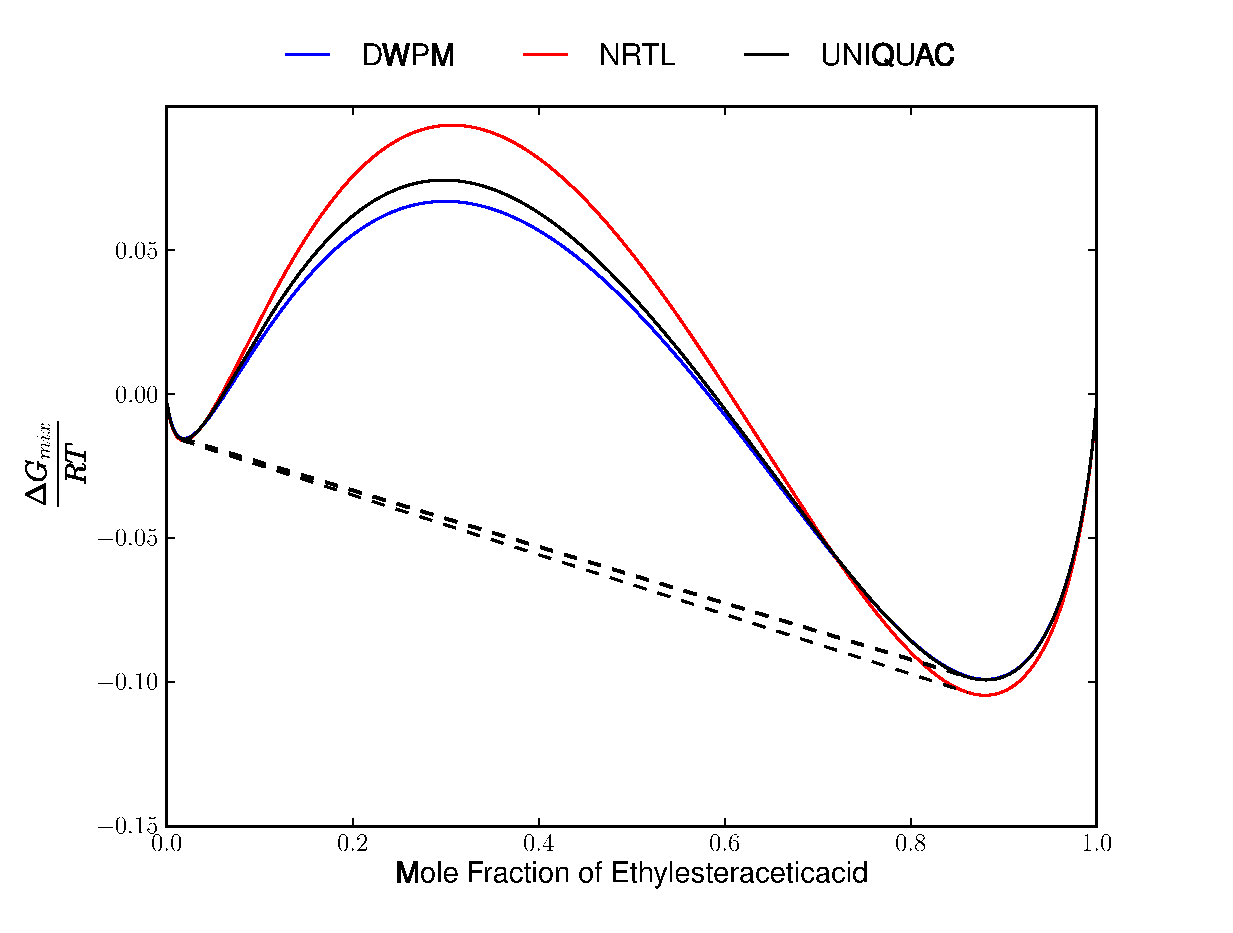
\includegraphics[width = \textwidth]{Results_Parts/BinaryParams/ethylesteraceticacid-water/AllModelsGibbsPlots/T_298.0.eps}
	\caption{298.0~$\mathrm{K}$}
\end{subfigure}%
\\%
\begin{subfigure}[h]{0.5\textwidth}
	\centering
	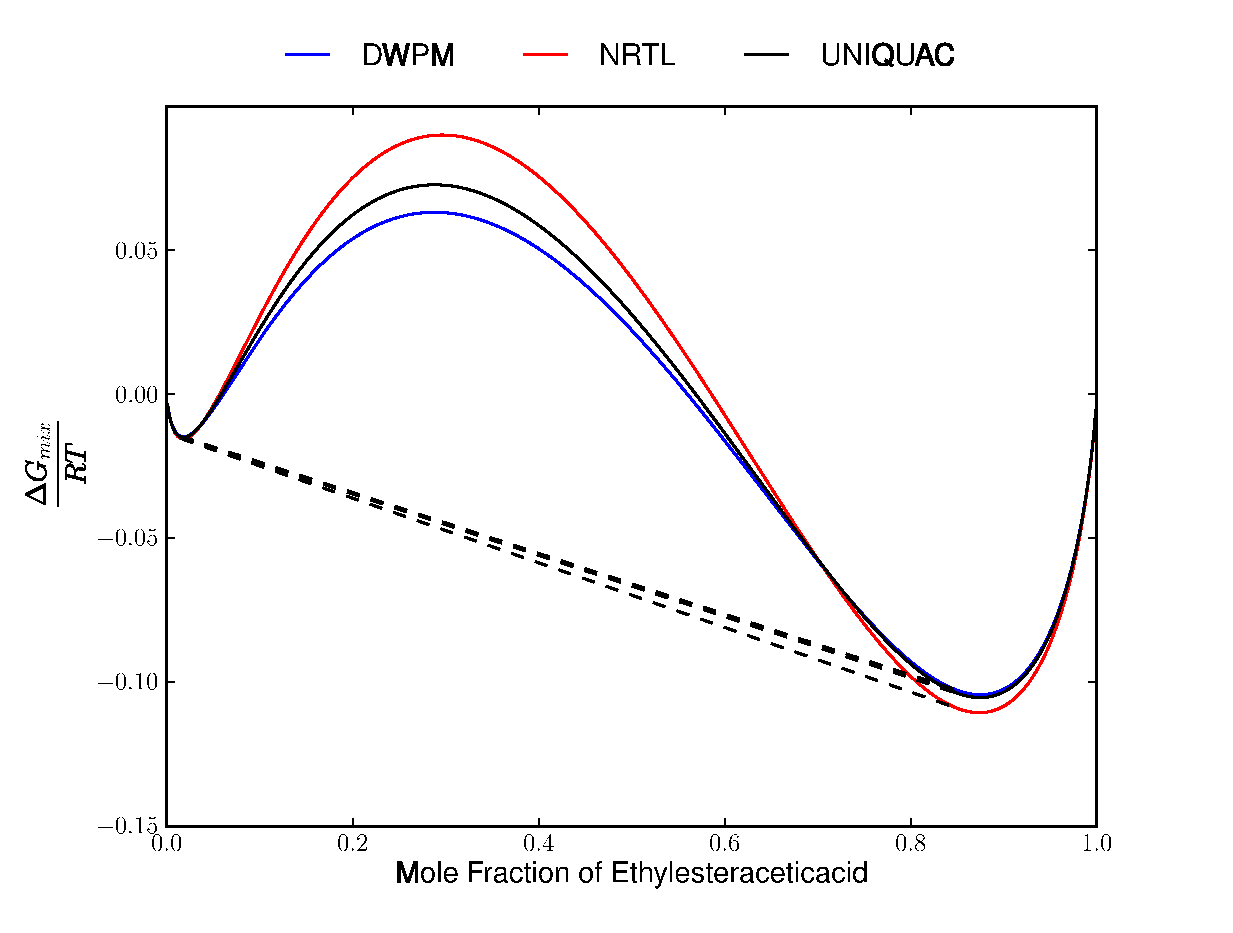
\includegraphics[width = \textwidth]{Results_Parts/BinaryParams/ethylesteraceticacid-water/AllModelsGibbsPlots/T_303.0.eps}
	\caption{303.0~$\mathrm{K}$}
\end{subfigure}%
~%
\begin{subfigure}[h]{0.5\textwidth}
	\centering
	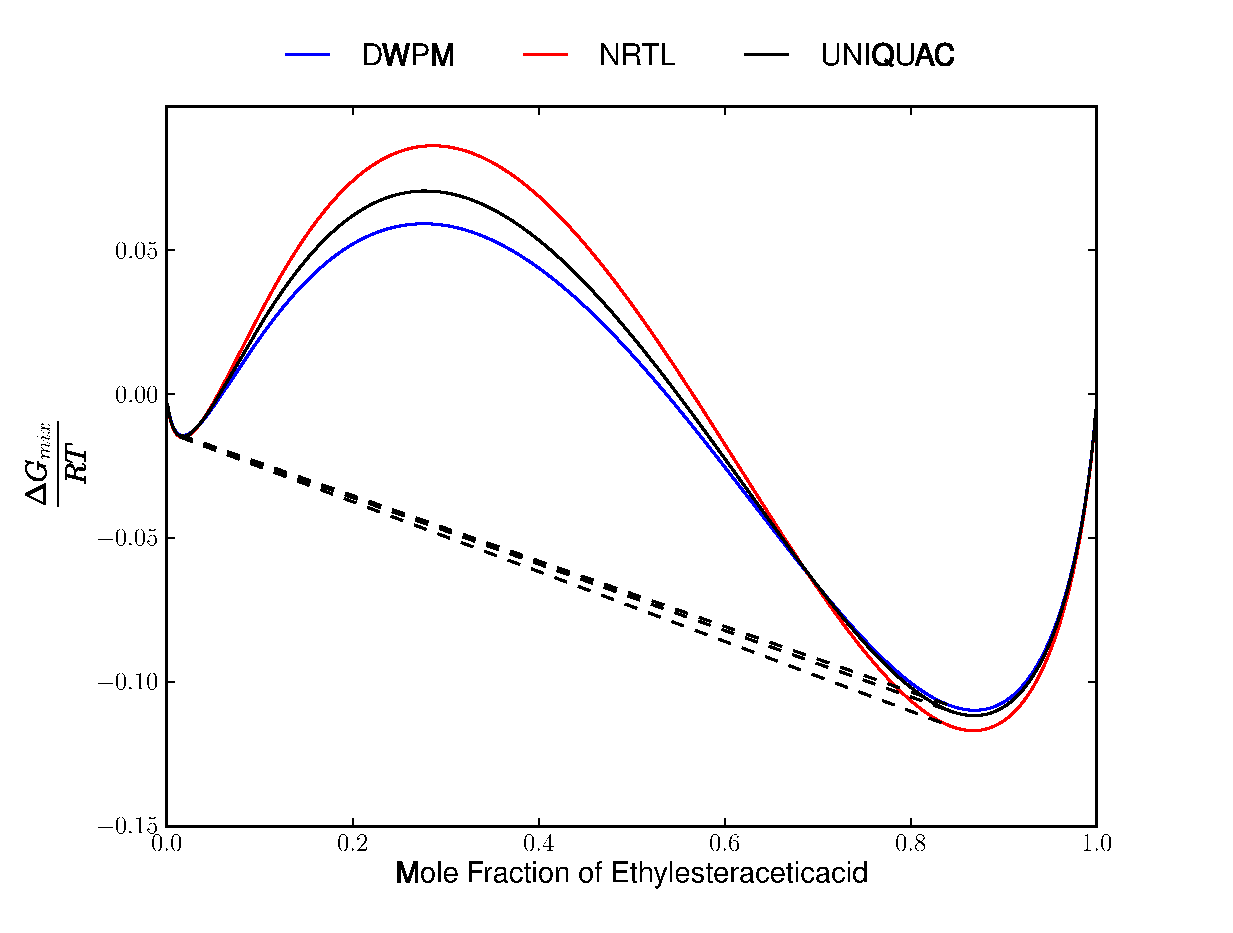
\includegraphics[width = \textwidth]{Results_Parts/BinaryParams/ethylesteraceticacid-water/AllModelsGibbsPlots/T_308.0.eps}
	\caption{308.0~$\mathrm{K}$}
\end{subfigure}%
\caption[]{Calculated liquid-liquid equilibrium for Ethyl Ester Acetic Acid and Water}
\end{figure}
\vspace*{\fill}
\clearpage
\begin{figure}[hpt]
\ContinuedFloat 
\begin{subfigure}[h]{0.5\textwidth}
	\centering
	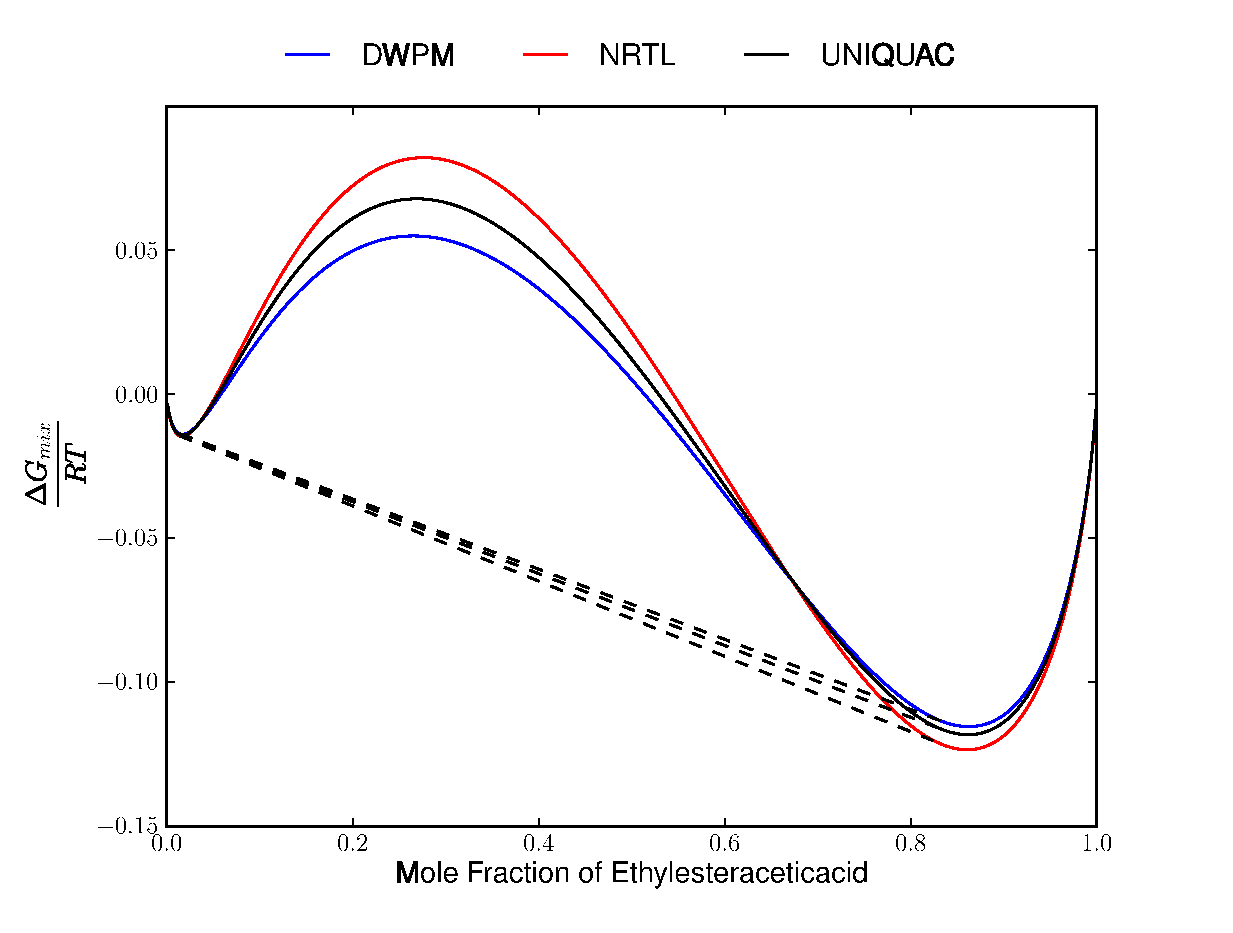
\includegraphics[width = \textwidth]{Results_Parts/BinaryParams/ethylesteraceticacid-water/AllModelsGibbsPlots/T_313.0.eps}
	\caption{313.0~$\mathrm{K}$}
\end{subfigure}%
\caption[]{Calculated liquid-liquid equilibrium for Ethyl Ester Acetic Acid and Water}
\end{figure}
\clearpage
%%----------------------------------------------------------------------------------------------------------------------------------------------%%

\subsection{Methanol and Heptane}
\vspace*{\fill}
\begin{figure}[hp]
\begin{subfigure}[h]{0.5\textwidth}
\centering
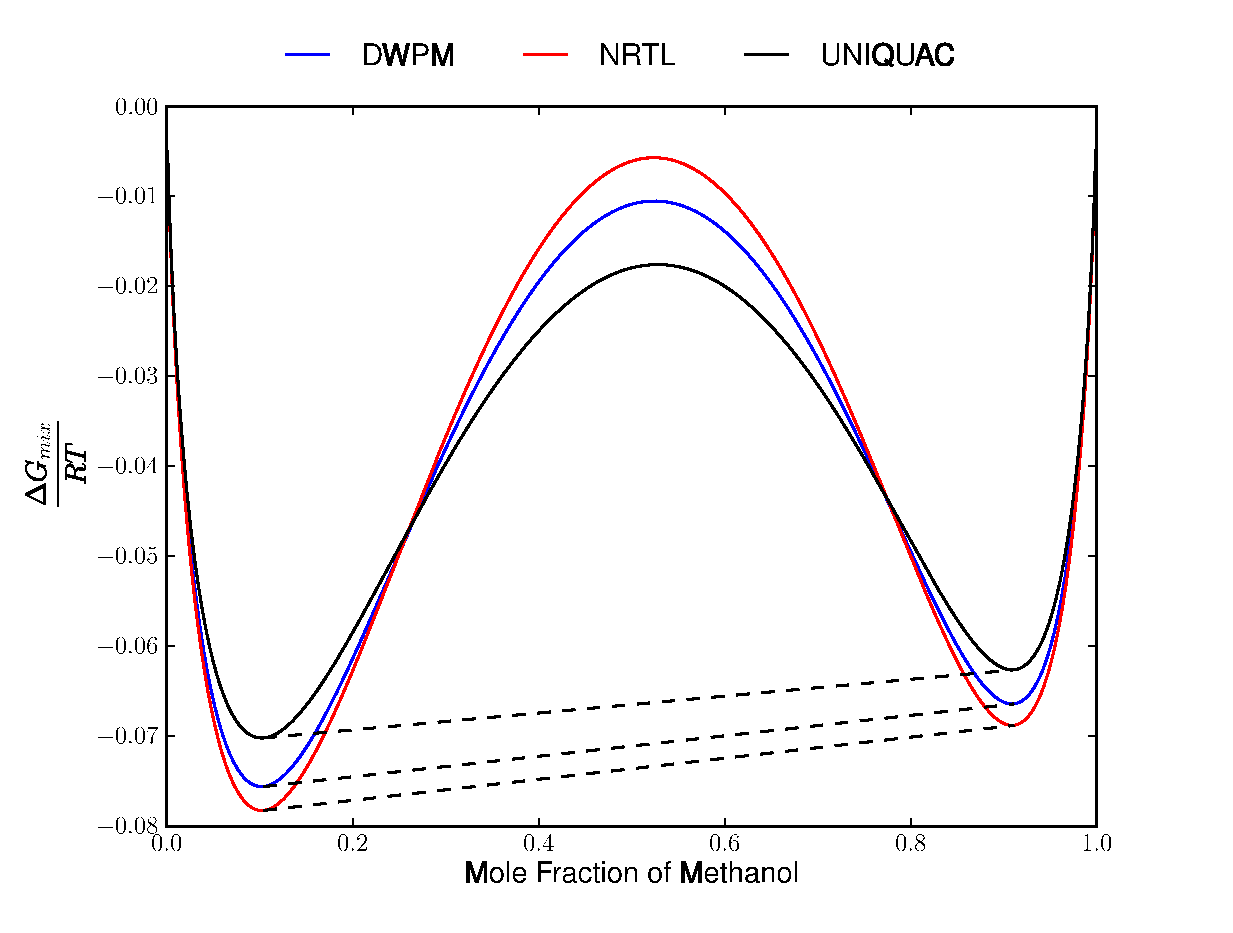
\includegraphics[width = \textwidth]{Results_Parts/BinaryParams/methanol-heptane/AllModelsGibbsPlots/T_291.eps}
\caption{291.0~$\mathrm{K}$} \label{methanol-heptane291}
\end{subfigure}%
~%
\begin{subfigure}[h]{0.5\textwidth}
\centering
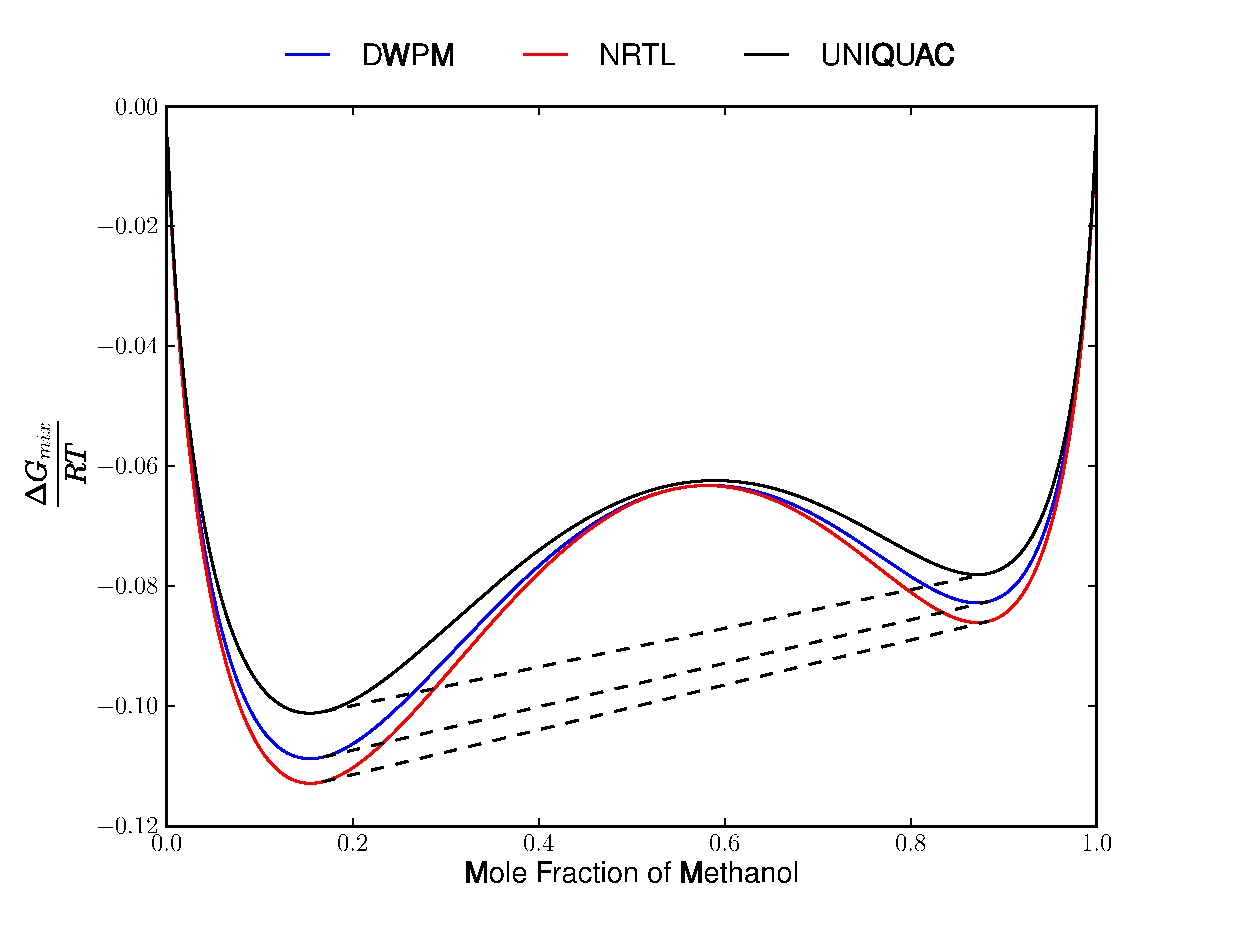
\includegraphics[width = \textwidth]{Results_Parts/BinaryParams/methanol-heptane/AllModelsGibbsPlots/T_303.eps}
\caption{303.0~$\mathrm{K}$} 
\end{subfigure}%
\\%
\begin{subfigure}[h]{0.5\textwidth}
\centering
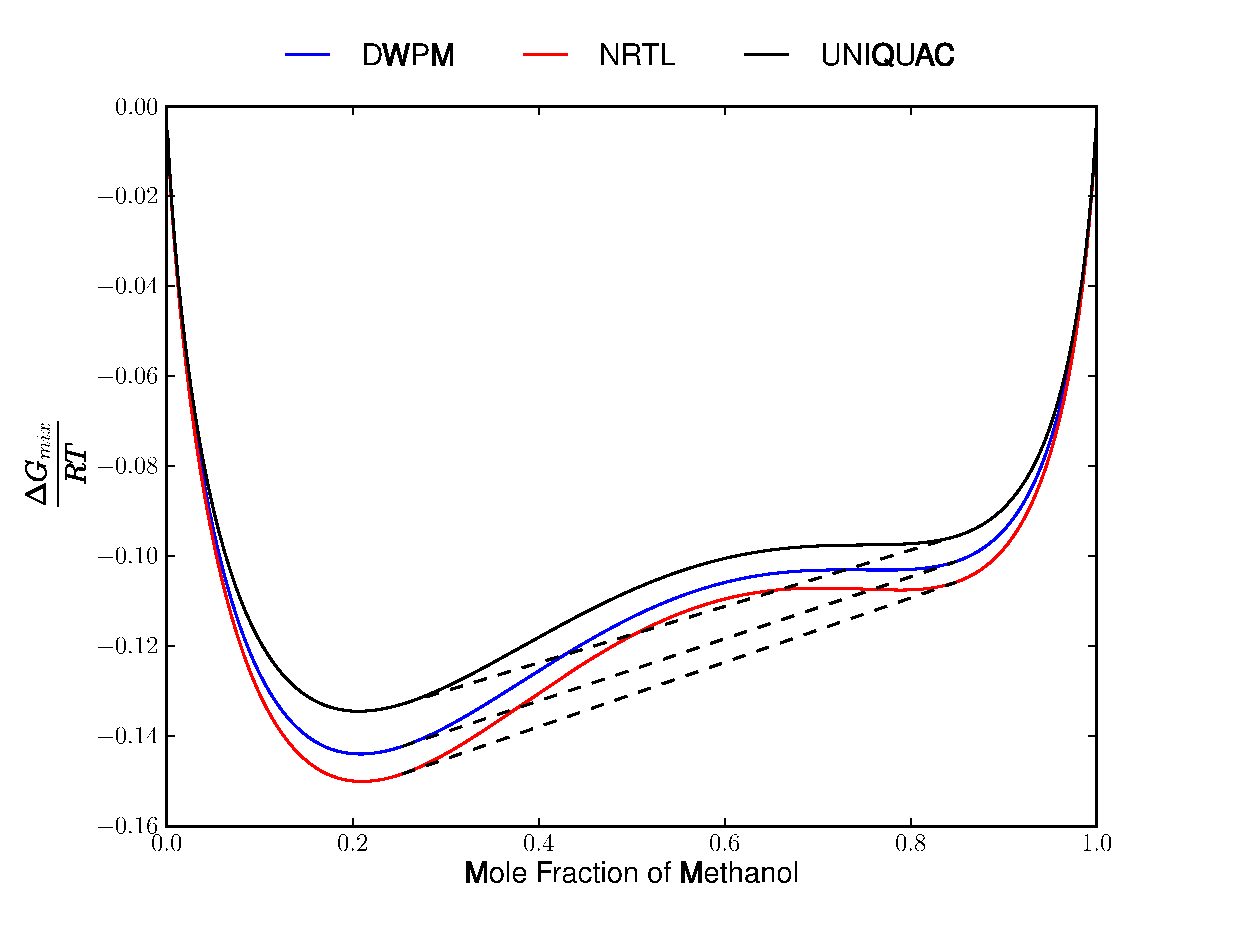
\includegraphics[width = \textwidth]{Results_Parts/BinaryParams/methanol-heptane/AllModelsGibbsPlots/T_313.eps}
\caption{313.0~$\mathrm{K}$} 
\end{subfigure}%
~%
\begin{subfigure}[h]{0.5\textwidth}
\centering
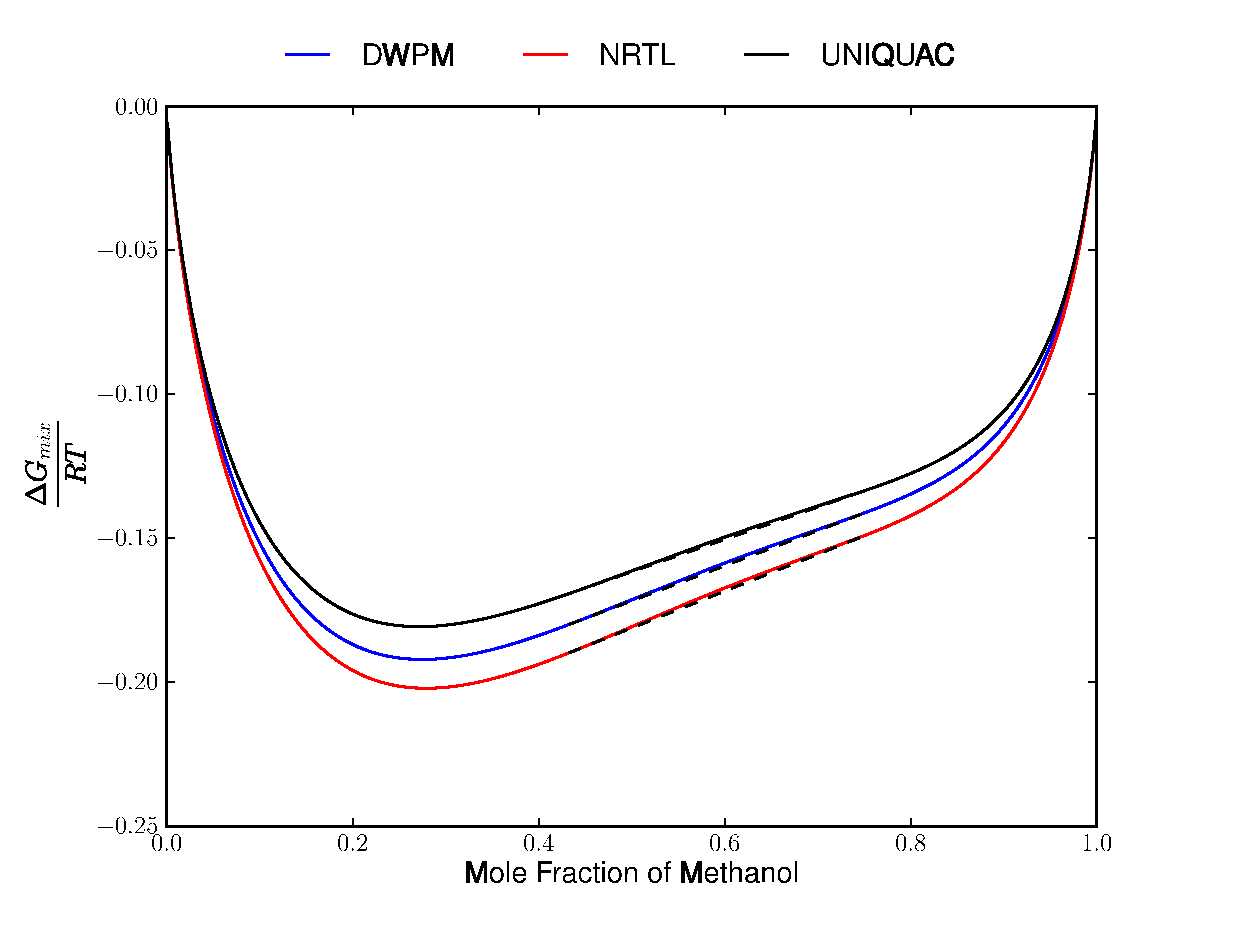
\includegraphics[width = \textwidth]{Results_Parts/BinaryParams/methanol-heptane/AllModelsGibbsPlots/T_323.eps}
\caption{323.0~$\mathrm{K}$} \label{methanol-heptane323}
\end{subfigure}%
\caption{Calculated liquid-liquid equilibrium for Methanol and Heptane}
\end{figure}
\vspace*{\fill}
\clearpage

%%-----------------------------------------------------------------------------------------------------------------------------------------------%%

\subsection{Methanol and Hexane}
\vspace*{\fill}
\begin{figure}[hp]
\begin{subfigure}[h]{0.5\textwidth}
\centering
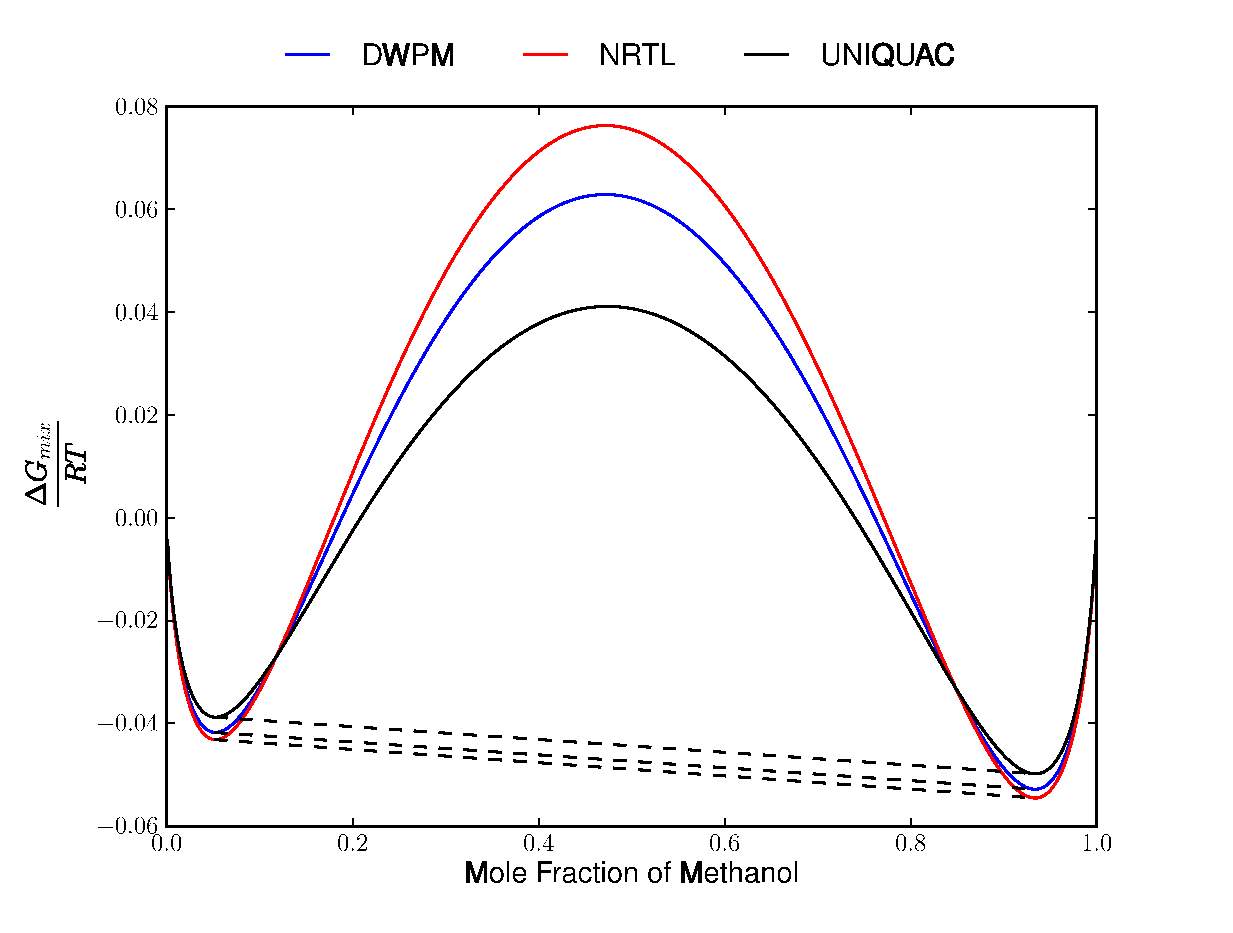
\includegraphics[width = \textwidth]{Results_Parts/BinaryParams/methanol-hexane/AllModelsGibbsPlots/T_255.2.eps}
\caption{255.2~$\mathrm{K}$} \label{methanol-hexane255}
\end{subfigure}%
~%
\begin{subfigure}[h]{0.5\textwidth}
\centering
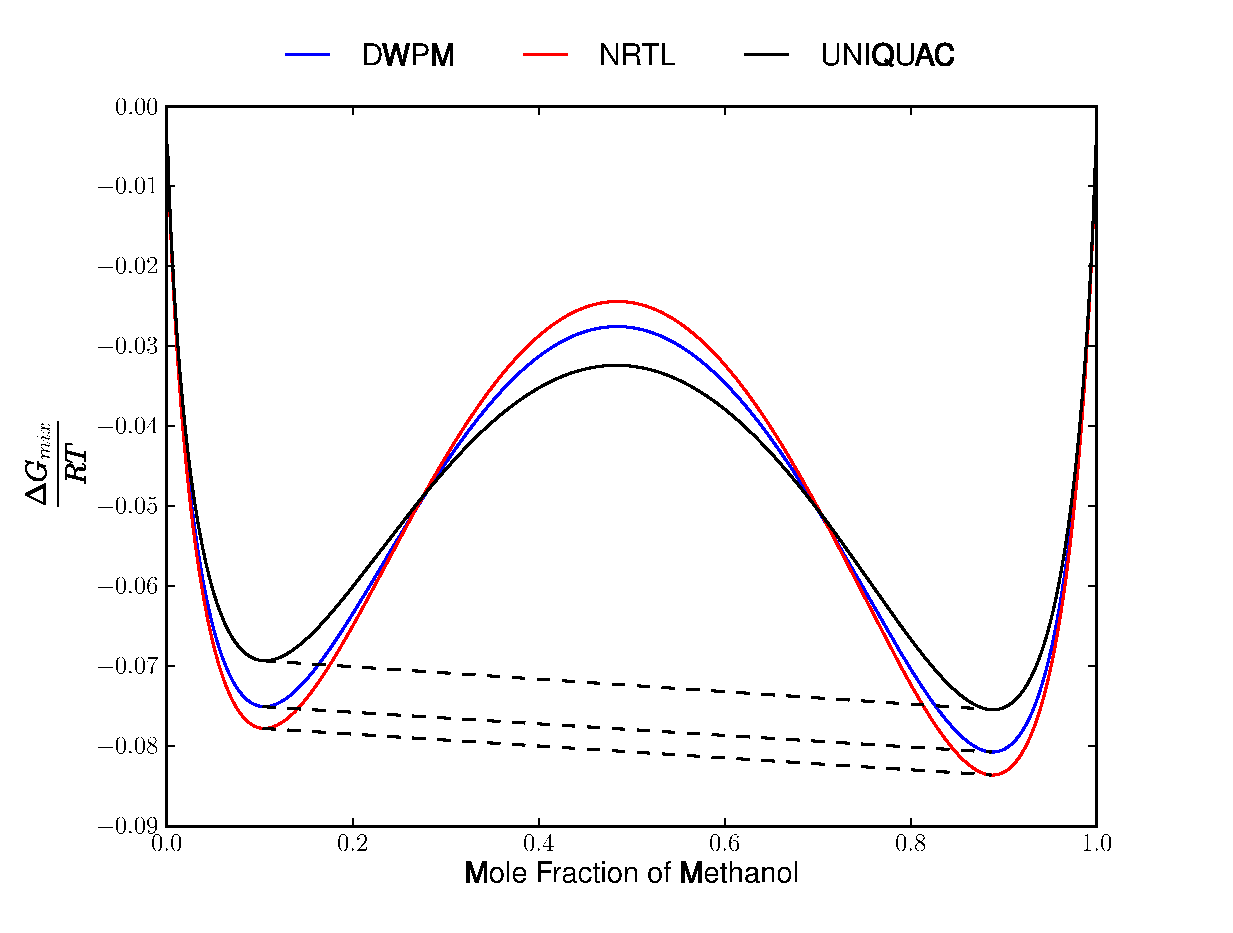
\includegraphics[width = \textwidth]{Results_Parts/BinaryParams/methanol-hexane/AllModelsGibbsPlots/T_278.0.eps}
\caption{278.0~$\mathrm{K}$} 
\end{subfigure}%
\\%
\begin{subfigure}[h]{0.5\textwidth}
\centering
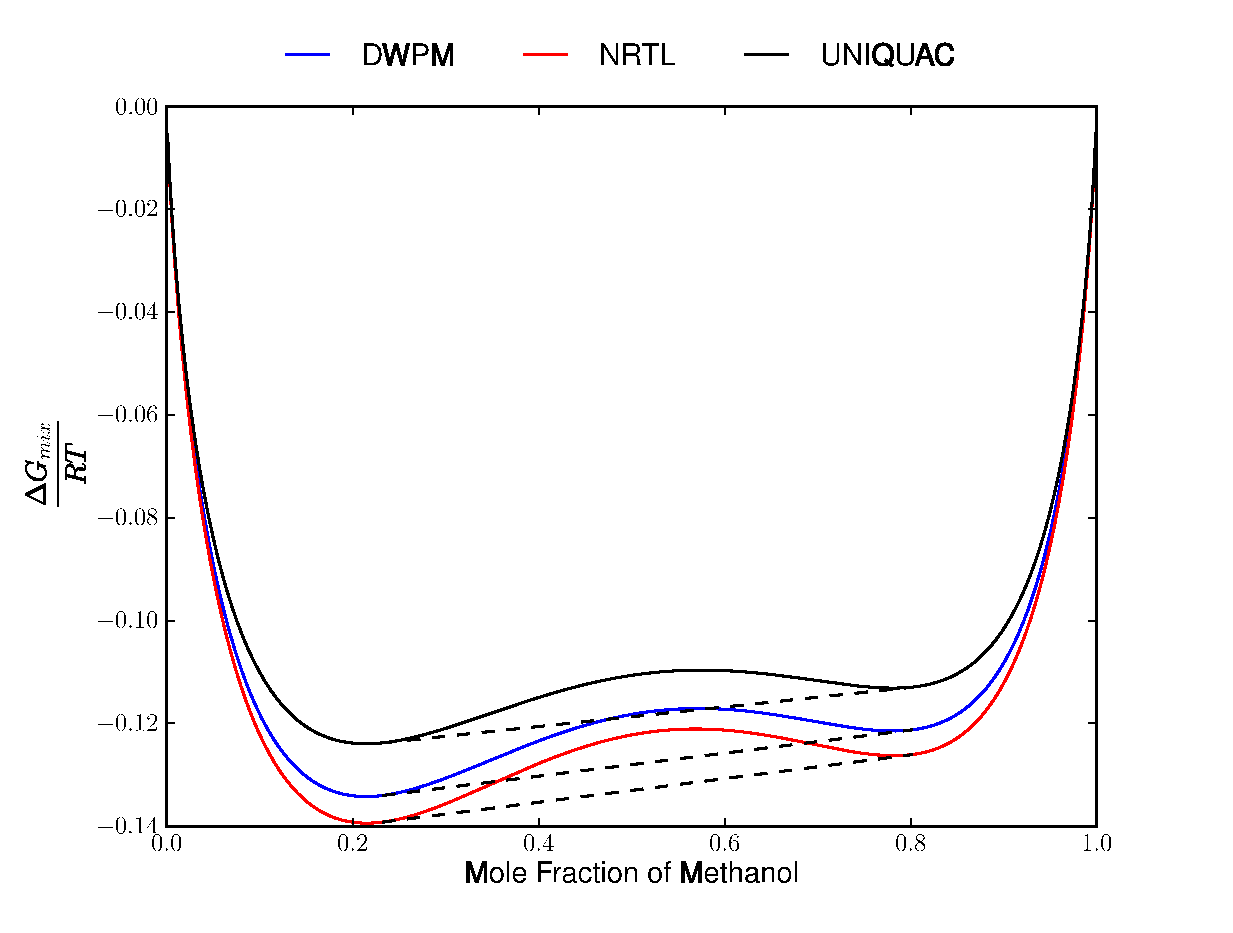
\includegraphics[width = \textwidth]{Results_Parts/BinaryParams/methanol-hexane/AllModelsGibbsPlots/T_298.0.eps}
\caption{298.0~$\mathrm{K}$} \label{methanol-hexane298}
\end{subfigure}%
\caption{Calculated liquid-liquid equilibrium for Methanol and Hexane}
\end{figure}
\vspace*{\fill}
\clearpage